\documentclass[12pt, a4paper, twoside]{article}

%% Preamble
\usepackage{umatfgspanish} % Estilo de la Universidad de Málaga
\usepackage[backend=biber]{biblatex} % Para la bibliografía
\addbibresource{bibliografia.bib} 
\usepackage{subfiles} % Best loaded last in the preamble
\usepackage{blindtext} % Para texto de relleno
\usepackage{verbatim} % Para comentarios
\usepackage{forest} % Para árboles
\usepackage{enumitem} % Para listas con símbolos personalizados
\usepackage{hyperref} % Para enlaces
\usepackage{dirtree} % Para estructura de directorios
\usetikzlibrary{arrows.meta}
\graphicspath{ {./images/} }



\begin{document}


%% Front Cover

\includepdf[noautoscale=true, width=\paperwidth]{Portada-Titulo-Contraportada/cover.pdf}
\newpage

%% Title Page

\includepdf[noautoscale=true, width=\paperwidth]{Portada-Titulo-Contraportada/title.pdf}

%% Abstract
\subfile{sections/abstract}
\newpage

%% Resumen
\subfile{sections/resumen}
\newpage

% Table of Contents
\tableofcontents
\newpage












%% Introduccion
\section{Introducción}
\label{sec:Introduccion}

\subsection{Motivación}
Las herramientas de automatización de tareas son fundamentales para la productividad en el desarrollo de software, permiten mejorar la eficiencia, la calidad y la consistencia en la producción de código.
Al relegar tareas repetitivas y propensas a errores a herramientas automatizadas, los desarrolladores pueden centrarse en tareas más creativas y de mayor valor añadido.

Parte del ciclo de vida en un desarrollo de software implica la configuración y el despliegue de servicios en entornos de producción y desarrollo.
La configuración y despliegue requiere de la creación de archivos de configuración específicos, como son, por ejemplo, los archivos \hyperref[sec:Dockerfile]{\emph{Dockerfile}} y \hyperref[sec:dockerignore]{\emph{.dockerignore}}, que definen cómo se construye la imagen de un contenedor en tecnologías como \hyperref[sec:Docker]{\emph{Docker}}.

En el contexto de la tecnología de contenedores, Docker se ha convertido en una de las plataformas más populares para la creación, el despliegue y la gestión de aplicaciones en entornos contenerizados. 
Sin embargo, la configuración de servicios en Docker puede ser una tarea compleja y propensa a errores, especialmente cuando se manejan múltiples servicios y configuraciones.

La motivación para realizar este proyecto surge de la necesidad de simplificar y automatizar el proceso de generación de archivos de configuración para el despliegue de servicios en Docker. 
En la actualidad, la creación manual de estos archivos Dockerfile puede ser una tarea repetitiva y susceptible a fallos al no conocer el usuario toda la información necesaria para la correcta configuración de los servicios.

Al desarrollar una herramienta que automatice este proceso, se busca mejorar la eficiencia y la precisión en la configuración de entornos de contenedores, facilitando así el trabajo de desarrollo y administración. 

\subsection{Objetivo}
La meta principal de este proyecto es desarrollar una herramienta que permita la generación automática de archivos de configuración para el despliegue de servicios en Docker.
Siguiendo las pautas recomendadas para la generación de dichos archivos mediante de plantillas, las plantillas han de ser extensibles y adaptables a los cambios en un futuro sin necesidad de reescribir código.
\\ \\
Para ello se plantean los siguientes objetivos específicos:
\begin{itemize}
	\item Investigar y analizar las tecnologías y herramientas existentes para la generación de archivos de configuración en Docker.
	\item Desarrollar una plantilla orientada a la generación de ficheros Dockerfile siguiendo las buenas prácticas.
	\item Implementar un modelo de plantillas extensible y adaptable a los cambios en las tecnologías y las metodologías de desarrollo.
	\item Desarrollar una herramienta web que permita la selección de plantillas y la generación de archivos de configuración para el despliegue de servicios en Docker.
	\item Desplegar la aplicación en un entorno no orientado a producción y documentar el proceso de instalación y uso.
	\item Evaluar la eficacia y la usabilidad de la herramienta en la memoria.
\end{itemize}

\newpage 
\subsection{Resultados Esperados}
Dada la gran cantidad de opciones de configuración disponibles para la generación de ficheros de configuración, el desarrollo de esta herramienta presenta varios desafíos técnicos y conceptuales.
El primero de ellos es la magnitud de las opciones de configuración disponibles, que pueden variar en función de las necesidades y los requisitos de cada servicio.
dar una cobertura a todos los escenarios posibles es una tarea inabarcable, por lo que se ha optado por centrarse en los casos de uso más comunes y en las configuraciones más utilizadas en la práctica.
Sin embargo, se espera que la herramienta sea lo suficientemente flexible y extensible como para permitir la incorporación de nuevas plantillas y configuraciones en el futuro.

Los desarrollos de los servicios resultantes de la implementación no tendrán el objetivo de alcanzar un estado de producción, sino de servir como base para futuras implementaciones y desarrollos orientados a ello. 

\subsection{Estructura del documento}

\begin{itemize}[label=\textbullet]
	\item El \hyperref[sec:Introduccion]{Capítulo 1 } describe la motivación del trabajo, sus objetivos, y los resultados esperados.
	\item El \hyperref[sec:Estado del Arte]{Capítulo 2 } presenta una breve introducción a los contenidos, al estado del arte, soluciones existentes y lo que se aporta en este contexto.
	\item El \hyperref[sec:Tecnologias Empleadas]{Capítulo 3 } describe las tecnologías y herramientas empleadas en el desarrollo del proyecto.
	\item El \hyperref[sec:Metodologia]{Capítulo 4 } describe la metodología de trabajo empleada en el desarrollo del proyecto.
	\item El \hyperref[sec:Modelado de las plantillas]{Capítulo 5 } desarrolla el modelado de las plantillas.
	\item El \hyperref[sec:Arquitectura y Descripción del sistema]{Capitulo 6 } define la arquitectura del proyecto y junto con la descripción de los servicios
	\item El \hyperref[sec:Extensibilidad]{Capítulo 7 } es un capítulo dedicado a la extensibilidad de las plantillas
	\item El \hyperref[sec:Despliegue de la aplicación]{Capítulo 8 }  describe el despliegue de la aplicación en un entorno no orientado a producción.
	\item El \hyperref[sec:Resultados]{Capítulo 9 } presenta los resultados obtenidos en el desarrollo del proyecto.
	\item El \hyperref[sec:Conclusiones]{Capítulo 10 } incluye las conclusiones del trabajo y las recomendaciones para trabajos futuros.
	\item El \hyperref[sec:Manual de Instalación]{Apéndice A} Es un manual de Instalación de la aplicación usando contenedores Docker.
	\item El \hyperref[sec:Manual de Uso]{Apéndice B} Es un manual de Uso de la aplicación web.
	\item El \hyperref[sec:Manual de Desarrollo]{Apéndice C} Es una guía para el desarrollo de plantillas, nuevas y existentes.
\end{itemize}




















%% Estado del Arte 
\section{Estado del Arte}
\label{sec:Estado del Arte}
Para comprender el sentido de este proyecto y su problemática es necesario contextualizar algunos conceptos previos que son necesarios para comprender la situación actual y reconocer los posibles problemas.
A continuación, se introducen dichos conceptos de manera escalonada, abordaremos la problemática de la generación de archivos de configuración en Docker, las tecnologías empleadas en la generación de dichos archivos y las soluciones actualmente disponibles.

\subsection{Contenedores}
Los contenedores son paquetes de software ligeros que incluyen el código de las aplicaciones junto con sus dependencias, como versiones concretas de entornos de ejecución de ciertos lenguajes de programación y bibliotecas para ejecutar los servicios de software~\cite{googlecontainers}.
\subsubsection{¿Por qué se usan los contenedores?}
Los contenedores constituyen un mecanismo de empaquetado lógico en el que las aplicaciones pueden extraerse del entorno en que realmente se ejecutan. 
Esta desvinculación facilita el despliegue uniforme de las aplicaciones basadas en ellos con independencia de que el entorno sea un centro de datos privado, la nube pública o el portátil personal de un desarrollador~\cite{googlecontainers}.
Es una solución de fácil aplicación, alto rendimiento y extremadamente portátil.\footnote{Existen restricciones en cuanto a la portabilidad de los contenedores, pero en general son fácilmente desplegables en cualquier entorno enlace:\href{https://stackoverflow.com/questions/42158596/can-windows-containers-be-hosted-on-linux}{https://stackoverflow.com/questions/42158596/can-windows-containers-be-hosted-on-linux}}.
\newpage

\subsection{Imágenes}
Las imágenes de contenedores son plantillas de solo lectura que contienen el código de la aplicación, las bibliotecas, las dependencias y otros archivos necesarios para ejecutar un contenedor~\cite{awsdocker}. 
No necesariamente necesitamos de una imagen para construir un contenedor\footnote{Existe la posibilidad de crear contenedores de otras formas, como a partir de otros contenedores.} pero ese es el escenario más común.\footnote{Construir un contenedor a partir de una imagen lo hace reproducible.}
\subsection{Docker}
\label{sec:Docker}
Docker \cite{docker} es una plataforma de código abierto que permite a los desarrolladores crear, desplegar y ejecutar aplicaciones en contenedores. Docker automatiza el despliegue de aplicaciones dentro de contenedores de software, proporcionando una capa adicional de abstracción y automatización de virtualización de aplicaciones en múltiples sistemas operativos.\footnote{Existen alternativas a Docker como Podman \cite{podman} pero Docker es la más popular y ampliamente utilizada en la actualidad.}
\subsubsection{Dockerfile}
\label{sec:Dockerfile}
El archivo Dockerfile \cite{dockerfile_concepts} es un archivo de texto que contiene una serie de instrucciones que Docker utilizará para construir una imagen de contenedor.
Usualmente, la construcción de un archivo de configuración se realiza a partir de una imagen base, que puede ser una imagen oficial de Docker o una imagen personalizada creada por el usuario.
A dicha imagen se le añaden las instrucciones necesarias para instalar las dependencias y configurar el entorno de ejecución de la aplicación, lo que viene a representar el contenido de un archivo Dockerfile.
\subsubsection{Dockerignore}
\label{sec:dockerignore}
El fichero .dockerignore \cite{dockerignore} es un tipo de archivo que puede colocarse en el proyecto del usuario y que se utiliza con la función de ignorar ficheros y directorios durante el \texttt{docker build}, con el objetivo de evitar que estos se copien a la imagen de Docker.
\newpage
\subsubsection{Buenas Prácticas en la creación de las imágenes}
Para la creación de los ficheros Dockerfile es recomendable seguir una serie de buenas prácticas para garantizar la eficiencia y la seguridad en el despliegue de servicios en Docker.
Estas prácticas se recogen en la documentación oficial de Docker \cite{dockerfile_best_practices}
En la documentación se abordan una serie de recomendaciones para la creación de imágenes de contenedores en Docker, entre las que se incluyen:
\begin{itemize}
    \item Utilizar imágenes oficiales de Docker:
    \begin{itemize}
        \item Las imágenes oficiales son mantenidas y actualizadas por la comunidad de Docker, lo que garantiza un alto nivel de seguridad y estabilidad.
        \item Estas imágenes suelen estar optimizadas para un rendimiento eficiente y son ampliamente documentadas.
    \end{itemize}
    
    \item Crea ficheros de configuración Multietapa:
    \begin{itemize}
        \item Crear imágenes en varias etapas permite dividir la construcción de la imagen, lo que puede mejorar el rendimiento.
        \item Esto ayuda a reducir el tamaño final de la imagen, incluyendo solo los archivos necesarios para la ejecución de la aplicación.
    \end{itemize}
    
    \item Usar una imagen base ligera:
    \begin{itemize}
        \item Utilizar imágenes base ligeras, como \texttt{`alpine'}, puede reducir significativamente el tamaño de la imagen Docker.
        \item Las imágenes ligeras también suelen tener menos vulnerabilidades de seguridad debido a su menor superficie de ataque.
    \end{itemize}
    
    \item Reducir el número de capas:
    \begin{itemize}
        \item Cada instrucción en un Dockerfile crea una nueva capa en la imagen. Reducir el número de capas puede mejorar el rendimiento y reducir el tamaño de la imagen.
        \item Combinar múltiples comandos en una sola instrucción \texttt{`RUN'} puede ayudar a minimizar el número de capas.
    \end{itemize}
    
    \item Eliminar archivos innecesarios:
    \begin{itemize}
        \item Durante el proceso de construcción, es importante eliminar cualquier archivo temporal o innecesario para mantener la imagen lo más pequeña posible.
    \end{itemize}
    
    \item Evitar el uso de la etiqueta \texttt{latest}:
    \begin{itemize}
        \item La etiqueta \texttt{latest} puede ser ambigua y llevar a problemas de consistencia y reproducibilidad.
        \item Es mejor especificar una versión concreta de la imagen para asegurar que se está utilizando la versión correcta.
    \end{itemize}
    
    \item Eliminar archivos temporales y de instalación:
    \begin{itemize}
        \item Durante la instalación de paquetes y dependencias, se generan archivos temporales que deben ser eliminados para reducir el tamaño de la imagen.
        \item Utilizar comandos como \texttt{`apt-get clean'} y \texttt{`rm -rf /var/lib/apt/lists/*'} para limpiar los archivos de instalación.
    \end{itemize}
    

    
\end{itemize}
\footnote{Para más información: \href{https://docs.docker.com/build/building/best-practices/}{https://docs.docker.com/build/building/best-practices/}}
\newpage 

\subsection{Problemática}
La dificultad de crear imágenes reside en la naturaleza de la aplicación que queremos llevar a un contenedor. Existen una gran cantidad de escenarios donde, si bien la tarea es sencilla, esta puede esconder una complejidad implícita de la que el usuario no es consciente. 
Estos apartados repercuten en el tiempo de compilación, tamaño de la imagen, mantenibilidad, seguridad y repetibilidad en las imágenes que se crean. \\
La calidad de las imágenes pueden marcar una diferencia que puede llegar a ser crítica para posteriores etapas en el desarrollo de aplicaciones, como son la Orquestación de contenedores \cite{ibm_container_orchestration}.

\subsection{Soluciones Actualmente Disponibles}
En la actualidad hay disponibles varias soluciones para disminuir la complejidad implícita que reside en la configuración de dichos ficheros Dockerfile. Existen más herramientas que las representadas a continuación, pero estas son las más empleadas.
\subsubsection{Docker init}
Docker init es el comando de Docker Desktop \cite{docker_desktop} que permite inicializar un proyecto con un archivo de configuración básico.
Su funcionamiento consta de elegir una plantilla de proyecto y seleccionar entre las opciones de configuración.
Las opciones de configuración se limitan a elegir el lenguaje de programación, puerto en el que despliega la aplicación y qué comando se ejecutará al iniciar el contenedor.
Las plantillas son creadas y mantenidas por la comunidad.\footnote{En este proyecto se reutilizan y se recogen ideas de varias de las plantillas que incluye Docker Init}
\begin{figure}[ht]
  \centering
    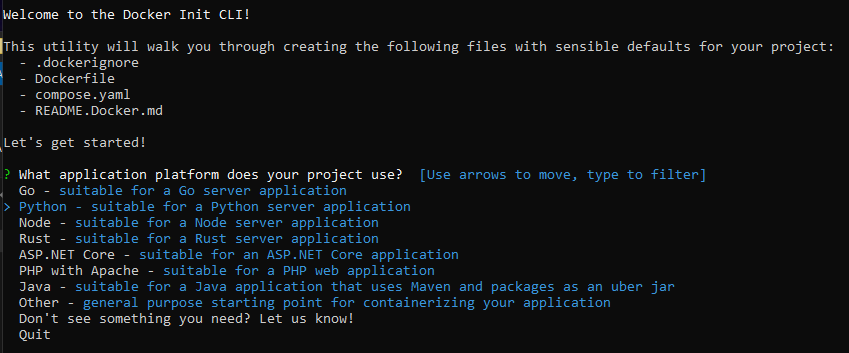
\includegraphics[width=1\textwidth]{Docker Init.png}
  \caption{Captura de las opciones de Plantillas disponibles Docker Init.}
\end{figure}

\newpage
\subsubsection{Docker Extension for Visual Studio Code}
La extensión de Docker para Visual Studio Code \cite{vscode_containers_overview} permite, entre otras muchas de sus funcionalidades, la generación del fichero Dockerfile entre otros.
Su comportamiento es similar al de Docker init, permitiendo, entre otras opciones, elegir el lenguaje de desarrollo del proyecto y qué comando se ejecutará al iniciar el contenedor.

\begin{figure}[ht]
	\centering
	  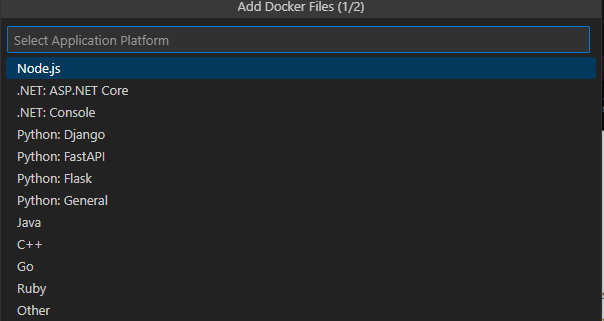
\includegraphics[width=1\textwidth]{Docker.extension.vscode.png}
	\caption{Plantillas Disponibles en la extensión para Docker de Visual Studio Code.}
\end{figure}

\begin{figure}[ht]
	\centering
		\includegraphics[width=1\textwidth]{docker.extension.vscode.Dockerfile.png}
	\caption{Captura de una plantilla generada por la extensión para Docker de Visual Studio Code.}
\end{figure}

\subsubsection{Inteligencia Artificial}
En la actualidad existen soluciones que se apoyan en la Inteligencia Artificial (IA) para la generación de archivos de configuración y para la creación de los ficheros Dockerfile. 
La calidad de estas soluciones es variable y depende de la calidad de los modelos de lenguaje natural empleados y de la calidad del \emph{prompt}.\footnote{Instrucción o texto inicial proporcionado a una herramienta generativa de IA para dirigir la generación de respuestas o resultados específicos \cite{panamericanlatam_prompt_ia}.} de entrada como \emph{magickpen} \cite{magickpen_dockerfile_template}\footnote{\href{https://magickpen.com/templates/128/}{magickpen: https://magickpen.com/templates/128/}.} o alternativas con propósito más general como \emph{chatgpt}. \cite{chatgpt} \footnote{\href{https://chat.openai.com/}{chatgpt: https://chat.openai.com/}.}

\begin{figure}[ht]
	\centering
		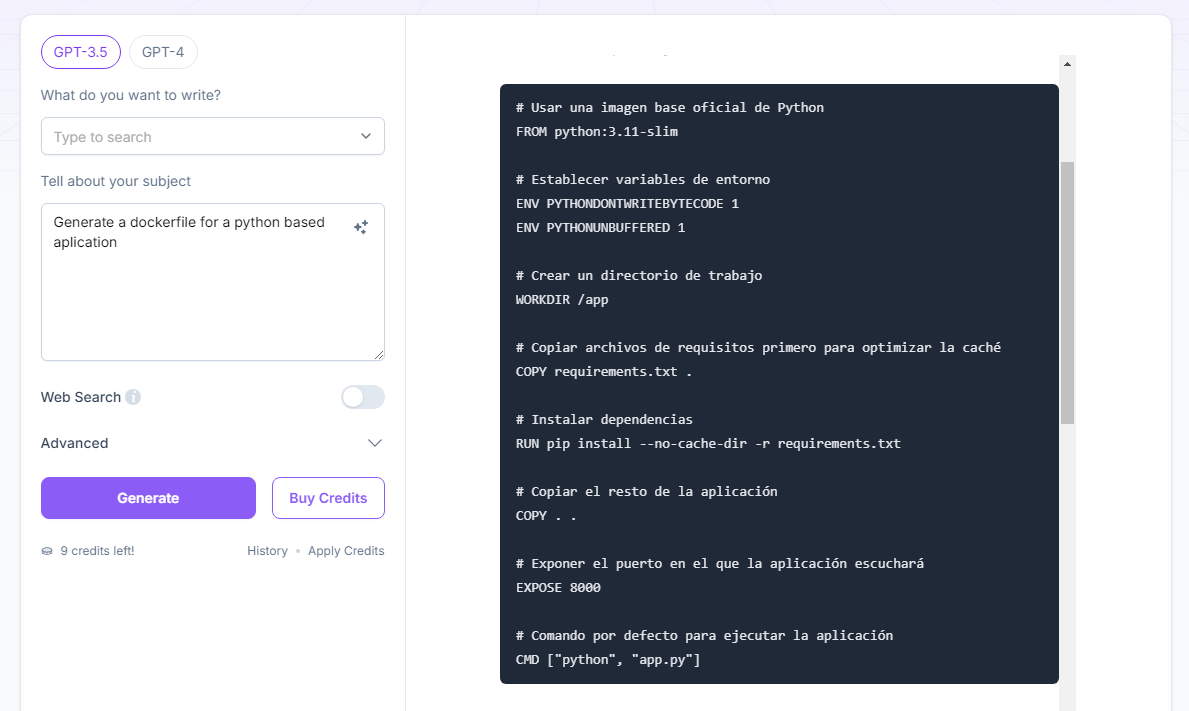
\includegraphics[width=1\textwidth]{MagickPen.png}
	\caption{Captura de un resultado de \emph{magickpen}.}
\end{figure}


\newpage
\subsection{Conclusiones Preliminares}
En este estudio se han recogido algunas de las principales herramientas y tecnologías disponibles en la actualidad para la generación de archivos de configuración.
Todas las herramientas (salvo propiamente los Modelos de Texto Generativo) hacen uso de plantillas para la generación de los ficheros Dockerfile y dockerignore, estas plantillas, si bien son correctas, son por naturaleza limitadas y no permiten la personalización final de las opciones de configuración.
No obstante, suponen un punto de partida para el desarrollo de aplicaciones contenerizadas. 

\subsection{¿Qué se aporta en este contexto?}
Las opciones actualmente disponibles para la generación de archivos de configuración para el despliegue de servicios en Docker son limitadas y no permiten la personalización de las opciones de configuración.
Se modela de forma separada la variabilidad y las posibles opciones que existen a la hora de construir las imágenes. El proyecto proporciona una nueva forma de construir plantillas, dotando capacidad al usuario de una personalización más profunda y detallada de las opciones de configuración de los servicios en Docker.
\subsubsection{Líneas de Producto Software (SPL)}
En el proyecto tendremos que construir nuestras propias plantillas que formarán parte de una línea de productos software.
Una línea de productos software (SPL del inglés \emph{Software Product Line}) es una familia de productos software relacionados entre sí que comparten ciertas características comunes (similitudes) pero que también tienen características variables.

En una SPL, los sistemas se descomponen en características (\emph{features}) que representan funcionalidades o comportamientos del sistema. 
El principal artefacto para modelar la variabilidad en SPLs son los modelos de variabilidad. Existen muchos modelos 
de variabilidad, pero los más extendidos y usados en la práctica son los modelos de características (\emph{feature models}). 

Un \emph{feature model} (FM) \cite{wikipedia_feature_model} es un modelo para representar la variabilidad de una SPL en base a características comunes y variables (véase Figura 1), especificando qué características se pueden seleccionar en una configuración para generar 
un producto válido de la SPL.  

\begin{figure}[ht]
	\centering
		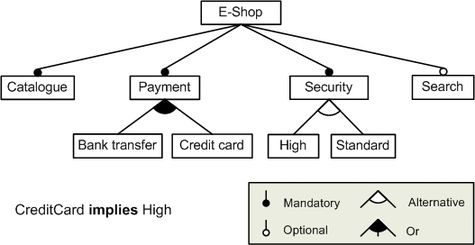
\includegraphics[width=0.75\textwidth]{fm.example.jpg}
	\caption{Ejemplo de representación gráfica de un \emph{feature model} \cite{wikipedia_feature_model}.}
\end{figure}












%% Tecnologías Empleadas
\section{Tecnologías Empleadas}
\label{sec:Tecnologias Empleadas}
Este apartado describe las tecnologías y herramientas empleadas más relevantes para el desarrollo del proyecto, así como su función y su relación con el objetivo del proyecto.

\subsection{Universal Variability Language (UVL)}

\emph{Universal Variability Language} (en adelante UVL) \cite{uvl} es un lenguaje de modelado diseñado específicamente para representar y manejar la variabilidad. 
La variabilidad en software se refiere a las partes de un sistema que pueden personalizarse, configurarse o cambiarse para adaptarse a diferentes necesidades o contextos. 
UVL se usa comúnmente en el contexto de ingeniería de líneas de productos software, donde se trabaja con una familia de productos que comparten un núcleo común, pero pueden tener variaciones.
Todas las plantillas que se han desarrollado en este proyecto requieren de un archivo UVL para poder generar configuraciones válidas.

\subsection{Docker}
La aplicación web, tanto como todos sus servicios, han sido desarrollados con el objetivo en mente de ser ejecutados dentro de contenedores.
Para el manejo de los contenedores en el entorno de desarrollo se ha optado por la utilización de Docker Desktop, un complemento con la consola de comandos.
Esta herramienta permite al proyecto hacerlo portable y fácil de desplegar en cualquier entorno.
\subsection{Node.js}
\cite{nodejs}
para el desarrollo de la aplicación web, se ha optado por la utilización de Node.js como entorno de ejecución de JavaScript para el desarrollo del Frontend.
Esta herramienta constituye una plataforma de desarrollo en tiempo de ejecución que tiene la ventaja de contar con una extensa biblioteca de módulos que simplifican el desarrollo de aplicaciones web.
Con npm (Node Package Manager) \cite{npm}, Node.js ofrece acceso a una vasta colección de paquetes y módulos que pueden ser fácilmente integrados en el proyecto, acelerando el desarrollo y reduciendo la necesidad de escribir código desde cero.
Para el proyecto se emplea la versión v22.10.0 y la versión v10.9.0 del gestor de paquetes npm.
\subsection{Angular}
\cite{angular}
En cuanto al desarrollo de la aplicación web, se ha optado por la utilización de Angular como framework de desarrollo.
El motivo de esta decisión es la idea de emplear un framework moderno que se usa con los métodos de desarrollo actuales y las mejores prácticas en el desarrollo de aplicaciones web.
Emplear otros frameworks de desarrollo como React o Vue.js también hubiera sido una opción válida al existir una cierta convergencia entre ellos en cuanto a funcionalidades y características.
Para los requisitos del proyecto, entendimos que Angular ya integra gran parte de las funcionalidades que requería nuestra aplicación ahorrando tiempo en la implementación de las mismas. La versión empleada es Angular v18.\footnote{Angular 18 no es la última versión disponible, pero al depender de otros desarrollos, se ha optado por la utilización de esta versión.}
\subsubsection{Angular Material}
\cite{angular_material}
Para el diseño de la interfaz gráfica de la aplicación web se ha optado por la utilización de los componentes provenientes de los módulos de Angular Material.
Siguiendo la línea de diseño de Material Design, Angular Material proporciona una serie de componentes y directivas que facilitan la creación de interfaces de usuario modernas y atractivas.
Los componentes tienen una interfaz conocida por el usuario y son fáciles de implementar en la aplicación web.\footnote{La última versión disponible es 18.2.9.}
\subsubsection{Monaco Editor}
\cite{monaco_editor} Para la edición de los archivos de configuración se ha optado por la utilización de Monaco Editor como editor de código.
Monaco Editor es un editor de código fuente basado en la web que se utiliza en varios proyectos de Microsoft, como Visual Studio Code, Azure DevOps y el editor de código de GitHub,
cuenta con una serie de características que lo hacen ideal para la edición de archivos de configuración, como el resaltado de sintaxis, el autocompletado y la verificación de errores.
también es altamente personalizable y extensible, lo que permite adaptarlo a las necesidades del proyecto.\footnote{La última versión de Angular con la que es compatible es la v18 por este motivo se ha desarrollado en esta versión de Angular \href{https://www.npmjs.com/package/ngx-monaco-editor-v2}{https://www.npmjs.com/package/ngx-monaco-editor-v2.}}
\subsubsection{ngx-json-viewer}
\cite{ngx_json_viewer}
Para la visualización de los archivos de configuración se ha optado por la utilización de ngx-json-viewer como visor de archivos JSON.
ngx-json-viewer es un componente de Angular que permite visualizar archivos JSON en un formato legible y estructurado. Es un proyecto de código abierto que se puede integrar fácilmente en aplicaciones Angular y personalizar según las necesidades del proyecto.

\subsection{Nginx}
\cite{nginx} 
Nginx es un servidor web de código abierto desarrollado en C que se utiliza para servir contenido web estático y dinámico, así como para actuar como proxy inverso y balanceador de carga.
la ventaja de Nginx es principalmente la poca necesidad de configuración que requiere para su correcto funcionamiento, además de ser un servidor web ligero y de alto rendimiento.
Para las necesidades del proyecto, se ha empleado en sus funciones de proxy inverso para redirigir las peticiones de la aplicación web al servidor de backend y como servidor web para servir el contenido estático de la aplicación web.

\subsection{Python}
\cite{python}
Python es un lenguaje de programación de alto nivel, interpretado y de propósito general que se ha convertido en uno de los lenguajes más populares en la actualidad.
Para el desarrollo de los servicios de backend se ha optado por la utilización de Python como lenguaje de programación.
Python es conocido por su sintaxis clara y legible, su amplia biblioteca estándar y su soporte para múltiples paradigmas de programación, como la programación orientada a objetos, la programación funcional y la programación imperativa.
\subsubsection{Flask}
\cite{flask}
Flask es un microframework de Python para el desarrollo de aplicaciones web.
Flask es conocido por su simplicidad y su facilidad de uso, lo que lo convierte en una excelente opción para el desarrollo de aplicaciones web pequeñas y medianas.
\subsubsection{Gunicorn}
\cite{gunicorn}
Gunicorn es un servidor HTTP WSGI para Python que se utiliza para servir aplicaciones web desarrolladas en Python. Su objetivo es proporcionar un servidor web simple y eficiente que pueda manejar múltiples solicitudes simultáneamente.
Esta herramienta es necesaria para el despliegue de la aplicación en un entorno de producción.
\subsubsection{Pypi}
\cite{pypi}
El uso de Pypi como repositorio de paquetes de Python es necesario para la instalación de las dependencias de la aplicación. Además, ha sido empleado para subir paquetes diseñados para la aplicación.

\subsection{Jinja}
\cite{jinja}
Jinja es un motor de plantillas para Python que se utiliza para generar archivos de texto dinámicos basados en plantillas. 

\subsubsection{Jinja2}
Jinja2 es la versión más reciente de Jinja y se utiliza comúnmente en aplicaciones web de Python para generar contenido dinámico.
Jinja2 es conocido por su sintaxis simple y legible, su capacidad para generar contenido dinámico y su integración con Python y otros marcos de desarrollo web.
Jinja2 permite la generación de archivos de texto dinámicos basados en plantillas, lo que facilita la creación de archivos de configuración personalizados y adaptables a las necesidades del usuario.
Todas las plantillas desarrolladas han usado la sintaxis de Jinja2.



\subsection{Git}
\cite{git}
Para el control de versiones se ha optado por la utilización de Git como sistema de control de versiones.
\subsection{GitHub}
\cite{github}
GitHub es una plataforma de desarrollo colaborativo que se utiliza para alojar proyectos de código, realizar seguimiento de problemas y tareas, y colaborar con otros desarrolladores.
Todo el proyecto es alojado en GitHub incluyendo plantillas, código, y demás recursos del proyecto.
\subsubsection{GitHub Public Api}
\cite{github_rest_api}
Para la gestión de las plantillas se ha empleado la API pública de GitHub para la obtención de las plantillas disponibles.
Esta decisión se ha tomado por facilidad de uso, ya que la API de GitHub es ampliamente conocida y documentada, y permite acceder a una gran cantidad de información sobre los repositorios y las plantillas disponibles.
Esto supone que las plantillas están visibles y son accesibles y modificables por cualquier usuario de GitHub.
Simplificando el proceso de creación, mantenimiento y actualización de las plantillas. 

\newpage

\subsection{Visual Studio Code}
\cite{vscode}
Visual Studio Code es un editor de código fuente desarrollado por Microsoft que se utiliza para escribir, editar y depurar código.
Su mención se debe a que es el editor de código fuente que se ha empleado para el desarrollo del proyecto. Además de ser clave en el proceso como generador de ficheros de configuración
de los que la aplicación hace uso.
\subsubsection{UVLS extension}
UVLS\cite{uvls_code} es una extensión de Visual Studio Code que proporciona soporte para UVL en el editor de código.
La extensión UVLS proporciona resaltado de sintaxis, autocompletado, verificación de errores y otras funcionalidades que facilitan la edición de archivos de configuración en UVL.
Además, la clave más importante es que es la única herramienta existente que permite crear una configuración correcta partiendo desde un \emph{feature model}.


Otras extensiones de menos importancia empleadas en \textit{VS Code} son:
\begin{itemize}
    \item \textbf{Docker Extension}
    \item \textbf{Flama}
    \item \textbf{Graphviz Interactive Preview}
    \item \textbf{Latex Workshop}
    \item \textbf{Pylance}
    \item \textbf{Python Debugger}
    \item \textbf{Better Jinja}
\end{itemize}














%% Metodología
\section{Metodología del trabajo}
\label{sec:Metodologia}
\subsection{Introducción}
El enfoque que se ha dado para abordar el desarrollo de este trabajo ha consistido en combinar un trabajo previo de análisis e investigación con una fase de desarrollo iterativo.

La investigación y análisis tenía el objetivo de conocer en profundidad las tecnologías y herramientas empleadas,
para posteriormente estudiar una posible aplicación de estas ideas y conceptos en el desarrollo de las plantillas.
Una vez resuelta esta primera parte, se ha procedido a una toma de requisitos y a la planificación de la implementación de la aplicación. Para la implementación de la aplicación, se ha optado por la utilización de una metodología de desarrollo que permita la evolución del proyecto a un producto mínimo viable en el menor tiempo posible.
\subsection{Metodología del Desarrollo}
Para la implementación del Proyecto se ha optado por un desarrollo en Cascada al tener una idea muy definida de lo que se quiere desarrollar y de las tecnologías empleadas.
Los cambios más relevantes surgen en las plantillas, es por ello que contamos con los mecanismos necesarios para adaptarnos a estos cambios sin que repercutan en el resto de la aplicación.
La implementación en cascada propone una serie de fases que se deben seguir de forma secuencial, pero para este escenario cada fase se inicia sin la necesidad de que la anterior haya sido completada, de forma que permita adaptarnos a requerimientos no planeados y encajar nuevas ideas que pudieran sucederse. En todo momento el código es susceptible de cambios.

\subsubsection{Justificación}
Al encontrarnos ante un trabajo individual, toda la responsabilidad y capacidad del desarrollo recae sobre una persona; esto supone una limitación en cuanto al contenido, pero supone una ventaja 
a la hora de adaptar cambios de la aplicación al centralizar todo el desarrollo en una persona. \\ 
El tiempo disponible es limitado por naturaleza y es vital simplificar todas las fases de la planificación del desarrollo. Por este motivo tenemos que descartar metodologías de desarrollo iterativo como Scrum y centrarnos en metodologías más rígidas como un desarrollo en Cascada.

El desarrollo de las plantillas requiere un estudio con el fin de limitar las opciones de configuración y centrarse en los casos de uso más comunes y en las configuraciones más utilizadas en la práctica.

\begin{figure}[ht]
	\centering
		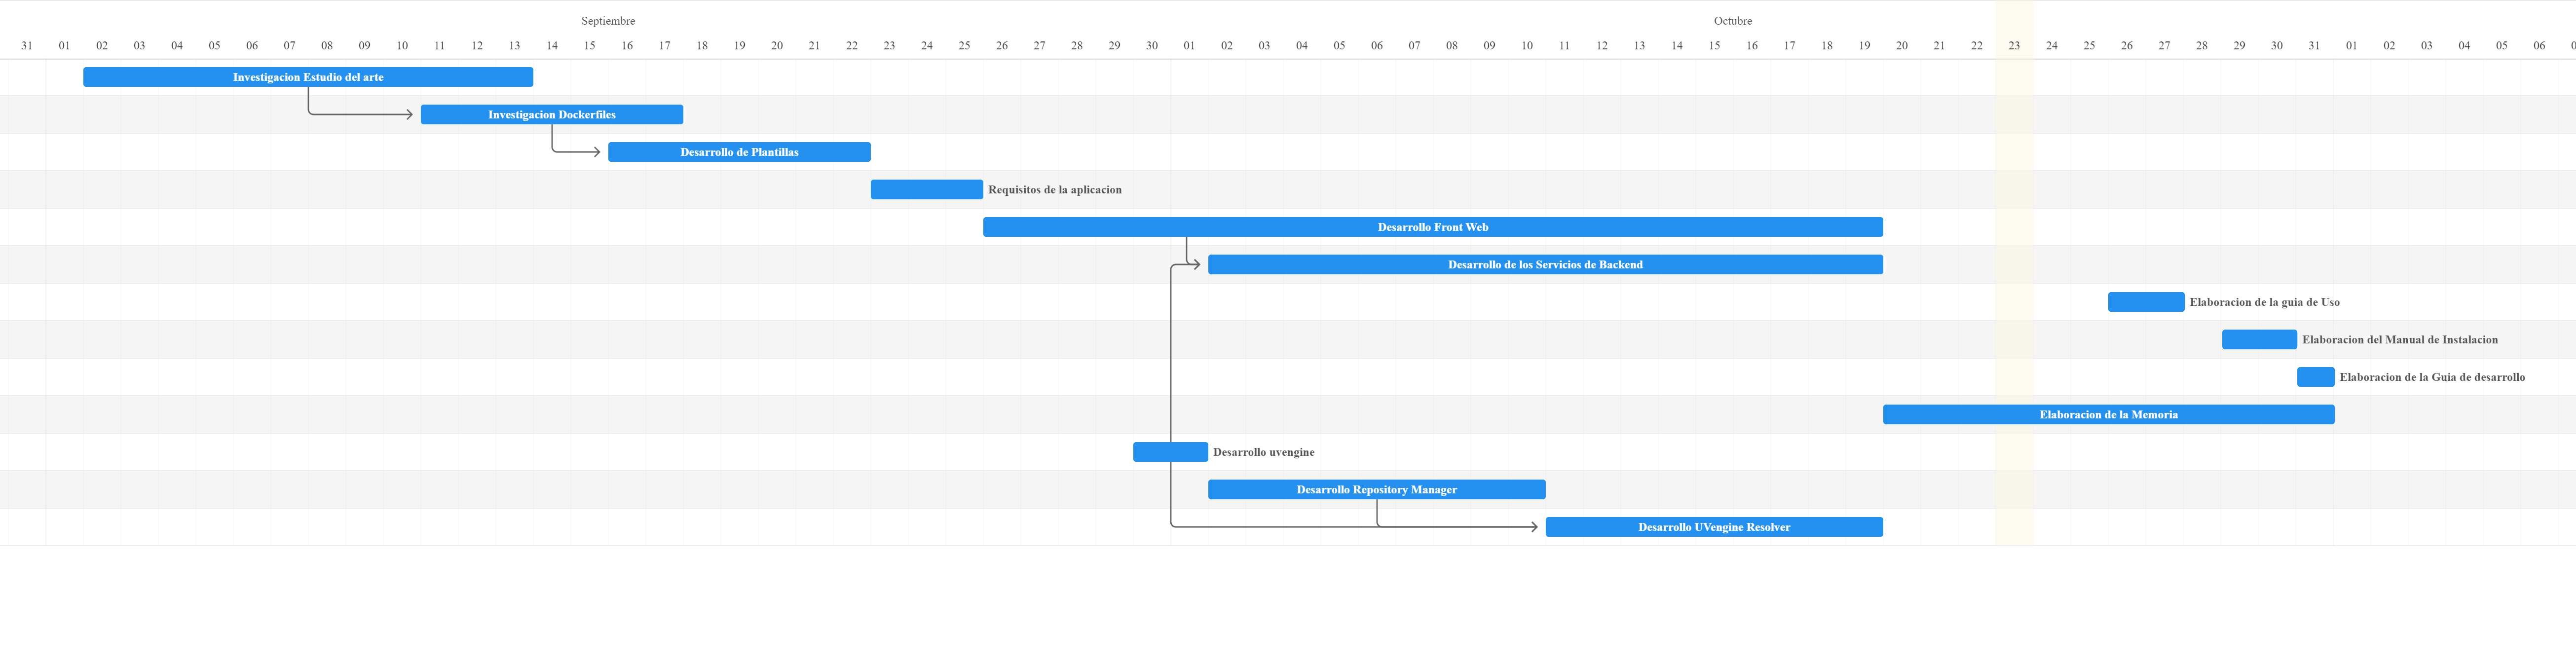
\includegraphics[width=1\textwidth]{gantt.png} 
	\caption{Diagrama de Gantt (generado por la herramienta \href{https://www.plandemejora.com/crear-diagrama-de-gantt-online/}{\emph{Diagrama de Gantt Online}}).} 
\end{figure}

\subsubsection{Notas del Procedimiento}
Se evaluaron con el tutor los momentos más relevantes, como los requisitos de la aplicación, arquitectura y una evaluación final, para introducir cambios que resultaron necesarios tanto en el proyecto como en la documentación y en las plantillas.

\subsubsection{Limitaciones}
El desarrollo de un proyecto de estas características requiere de una planificación y una metodología de trabajo adecuadas.
En este sentido, como se ha mencionado anteriormente, se identificaron una serie de limitaciones y restricciones que pueden afectar al desarrollo del proyecto.
En este sentido, el desarrollo de las plantillas tuvo que limitarse en cuanto a formato y contenido, ya que no se pueden abarcar todas las posibles opciones de configuración.
\\El tiempo que se puede dedicar al proyecto tiene que estar dentro de unos límites razonables para un trabajo de estas características y no se puede extender indefinidamente.

\subsection{Fases de Estudio}

\subsection{Estudio del Estado del Arte:}
En esta fase se realiza una revisión exhaustiva de la literatura y tecnologías existentes relacionadas con el tema del 
proyecto. El objetivo es comprender el panorama actual, identificar tendencias, mejores prácticas y tecnologías 
relevantes que puedan influir en el desarrollo del proyecto. Los puntos clave de esta fase son:

\begin{itemize}
	\item Para comprender la tecnología de los contenedores fue esencial la lectura de \href{https://www.oreilly.com/library/view/docker-certified-associate/9781839211898/c5ecd7bc-b7ed-4303-89a8-e487c6a220ed.xhtml#uuid-1a5da664-fb76-4e56-bdb0-83255dde9e78}{Modern Infrastructures and Applications with Docker}. \cite{docker_certified_associate}
	\item Completar la introducción al lenguaje UVL con \href{https://uvl.uni-ulm.de/}{UVL Playground} \cite{uvl_playground}.
\end{itemize}

\subsection{Investigación diseño de Dockerfiles}
Esta fase implica investigar y evaluar las diferentes opciones de configuración que se presentan en el desarrollo de un fichero Dockerfile en el 
despliegue de aplicaciones. Se exploran las características, herramientas y técnicas que pueden optimizar el uso de 
Docker en un proyecto software. 

\begin{itemize}
	\item Para comprender la importancia de las buenas prácticas en la creación de imágenes, fue necesario la lectura de la documentación oficial de Docker \href{https://docs.docker.com/reference/Dockerfile/}{Dockerfile reference} \cite{dockerfile_reference}.
\end{itemize}


\subsection{Desarrollo de Plantillas}
Esta fase implica la construcción del árbol de características y las restricciones textuales que orienten el espacio de 
configuraciones posibles del fichero Dockerfile. En este paso se ponen en práctica todo el conocimiento adquirido en los pasos anteriores que 
como resultado se obtiene el modelado de unas plantillas. Hemos de tener en cuenta las buenas prácticas y las recomendaciones de la comunidad para la creación de los ficheros Dockerfile \cite{dockerfile_concepts}. 
Estas prácticas tienen que estar presentes en el diseño de las plantillas desde el inicio, también hemos de generar test para mantener la consistencia de las implementaciones. 
Esta fase queda cubierta con más detalle en el \hyperref[sec:Modelado de las plantillas]{Capítulo 5}.


\subsection{Fase Implementación}
\subsubsection{Requisitos de la aplicación }
En esta sección se documentan los requisitos funcionales de la aplicación, obviando los requisitos no funcionales. Los requisitos han cambiado conforme el proyecto avanzaba en sus etapas de desarrollo
sin ánimo de ser exhaustivos, las funcionalidades mínimas que se pretenden alcanzar en cuanto a la generación de productos son:
\begin{itemize}
	\item La herramienta debe permitir seleccionar la plantilla y la versión con la que se desea trabajar. 
	\item Dentro de la aplicación se podrá recargar con nuevas plantillas que configuremos en un repositorio.
	\item La herramienta debe generar el producto en el momento en el que se aplique una configuración válida. 
	\item La herramienta debe permitir la descarga o copia al portapapeles del producto generado.
	\item La herramienta debe permitir la visualización de los archivos de configuración generados.
	\item La herramienta debe permitir la edición de los archivos de configuración generados.
	\item La herramienta debe de ser una solución portable a otros sistemas operativos.
\end{itemize}

\newpage 
\subsubsection{Diseño de la aplicación}
En esta fase se diseña la arquitectura de la aplicación, se definen los componentes y módulos que la componen y se establecen las relaciones entre ellos. 
En esta imagen se resumen los componentes de la aplicación. Una explicación más detallada puede encontrarse en el \hyperref[sec:Arquitectura y Descripción del sistema]{Capítulo 6}
\begin{figure}[h]
	\centering
		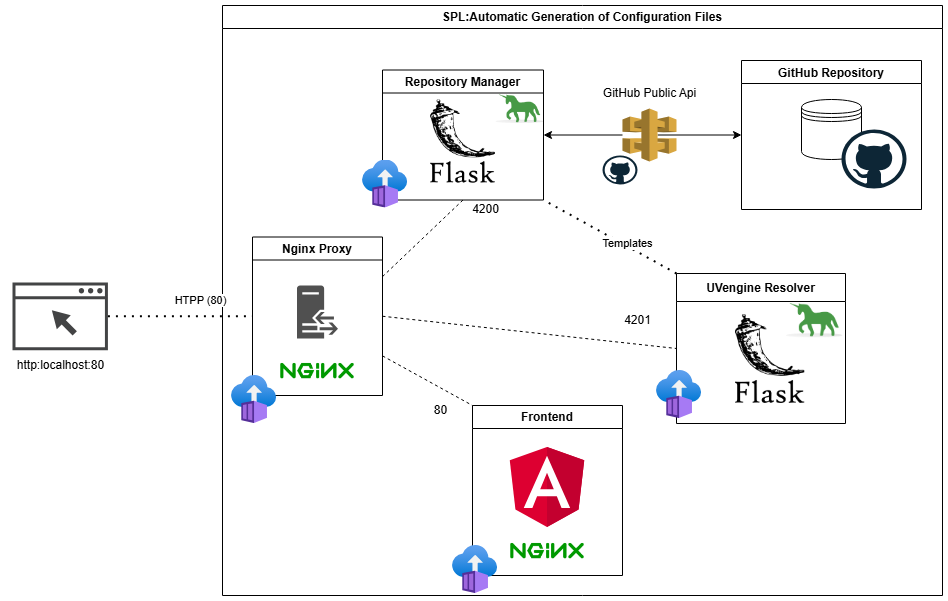
\includegraphics[width=1\textwidth]{Arquitectura Contenedores.png}
	\caption{Diagrama de infraestructura.} 
\end{figure}
\subsubsection{Desarrollo del Paquete UVEngine}
En esta fase se adapta el proyecto de la aplicación de UVEngine \cite{uvengine_github}, que permite la generación automática de archivos de configuración.
La adaptación consiste en hacer opcional el fichero mapping model \footnote{Mapping model:\hyperref[sec:Mapping Model]{Capítulo 5}} a la hora de generar un producto. Una vez adaptado, se procede a la creación de un paquete de Python que se pueda instalar en cualquier entorno de desarrollo.
como resultado, tenemos el paquete UVEngine. \cite{uvengine_pypi}\footnote{El paquete es empleado en el proyecto UVEngine-Resolver y en los entornos de desarrollo de las plantillas.}
\subsubsection{Desarrollo aplicación Frontend Angular}
En esta fase se desarrolla la aplicación web que permite la interacción con el usuario y la visualización de los archivos de configuración generados. Como hemos mencionado anteriormente, consta de un proyecto Angular presente en el siguiente repositorio GitHub \cite{m4rdom_frontend}.
La idea fundamental es permitir al usuario elegir entre un abanico de plantillas y versiones para que pueda decidir qué producto generar en base a la configuración que se aporte como entrada.
Debe funcionar como una abstracción de los servicios de Backend para permitir al usuario trabajar desde una interfaz web.
Angular utiliza un enfoque basado en componentes para la construcción de aplicaciones web, los componentes más relevantes son:
\begin{itemize}
	\item \texttt{Common Components/} contiene los componentes que se emplean en toda la aplicación.
	\item \texttt{Pages/} contiene los componentes que representan las páginas de la aplicación.
	\item \texttt{Services/} contiene los servicios que se emplean en la aplicación.
	\item \texttt{Shared Components/} contiene los componentes que se emplean específicamente para la integración con el editor de mocano.
	\item \texttt{Structure/} contiene los componentes que representan la estructura de la aplicación.
\end{itemize}

No olvidemos que gran parte de la lógica de la aplicación se encuentra desarrollada como servicios de la aplicación bajo el directorio \texttt{Service/}: 

\begin{itemize}
	\item \texttt{Services/} contiene los servicios que se emplean en la aplicación, como manejar las peticiones a backend y reescribir por pantalla los resultados.
\end{itemize}

\subsubsection{Desarrollo de los servicios de backend}
\label{sec:Desarrollo de los servicios de backend}
En esta fase se desarrollan los servicios de backend que permiten la comunicación entre la aplicación web y la aplicación de UVEngine y los repositorios.
El primer servidor de backend que vamos a generar será un servidor para gestionar las peticiones sobre las plantillas, a este servicio lo llamaremos \texttt{Repository-Manager}. 
Consiste en un servicio Flask que traduce las peticiones a la API de GitHub y las devuelve a la aplicación web. Desde este servicio tendremos acceso a la lista de plantillas y la lista de versiones.
Además, aportamos al siguiente servicio un método para la descarga de las plantillas. El siguiente servicio es el encargado de resolver la variabilidad de una configuración y generar un producto, a este servicio lo llamaremos \texttt{UVEngine-Resolver}.
Este servicio se encarga de la generación de productos a partir de una configuración válida; para ello se apoya en el paquete UVEngine que hemos desarrollado en la fase anterior.

\subsubsection{Elaboración de la guía de uso}
En esta fase se elabora una guía de uso que explica cómo utilizar la aplicación y las funcionalidades disponibles.
Se elabora una guía detallada que describe cómo utilizar la aplicación, incluyendo instrucciones paso a paso, capturas 
de pantalla y ejemplos. 
\subsubsection{Elaboración de un manual de instalación}
En esta sección se crea un manual de instalación que explica cómo instalar y configurar la aplicación en un entorno local.
\subsubsection{Elaboración de un manual de desarrollo de plantillas}
En esta parte se crea un manual de desarrollo de plantillas que explica cómo crear y mantener plantillas en el repositorio\footnote{\href{https://github.com/M4rdom/Templates}{https://github.com/M4rdom/Templates}}.
\subsection{Elaboración de la memoria}
En esta fase se redacta la memoria o informe final del proyecto, que documenta todo el proceso de desarrollo, desde la 
planificación hasta la implementación y las lecciones aprendidas. La memoria incluirá el análisis de los resultados, 
conclusiones y recomendaciones para trabajos futuros. 



















%% Modelado de las plantillas
\section{Modelado de las plantillas}
\label{sec:Modelado de las plantillas}
Este espacio pretende describir de forma detallada el modelado de las plantillas y a qué necesidad responden en la construcción de un fichero de configuración.
\subsection{Introducción}
Dar cabida a la gran cantidad de escenarios y posibles casos de uso para la aplicación se ha descrito anteriormente como una tarea abrumadora.
Aunque pudiéramos crear una plantilla lo suficientemente expresiva para dar cabida a todos los escenarios de uso existentes hasta la fecha, las plantillas quedarían desfasadas conforme se suceden cambios 
en las metodologías, surgen nuevas imágenes base, otras quedan desactualizadas, etc. La obra resultante llegaría a ser impracticable en cuanto a la cantidad de opciones y configuraciones que se podrían dar.
El objetivo del desarrollo de todas las plantillas de este proyecto no pretende llegar a un nivel extremadamente avanzado de personalización, sino que sirvan como base para la creación de plantillas más específicas y detalladas.

\newpage

\subsection{Componentes de las plantillas}
\subsubsection{Feature model}
El archivo .uvl es el archivo principal de la plantilla, contiene la descripción de las características y las restricciones de la plantilla.
Este archivo lo usará la extensión UVLS \cite{uvls_code} para generar una configuración válida que cumpla con las restricciones textuales que dictemos en el archivo, de este modo nos aseguramos de que estamos aplicando una configuración válida.
\begin{figure}[ht]
	\centering
		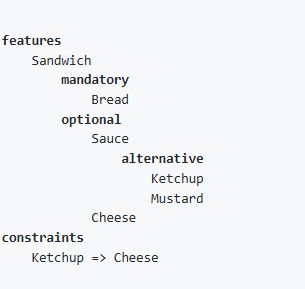
\includegraphics[width=0.5\textwidth]{text.feature_model.png}
	\caption{Representación de un Feature model en lenguaje UVL \cite{uvl}.}
\end{figure}

\newpage

\subsubsection{Plantillas Jinja}
Las plantillas Jinja son los archivos de plantilla que se utilizan para generar los productos a partir de una configuración válida del modelo.
La idea es exponer estas plantillas ante una configuración ya validada usando UVLS \cite{uvls_code}. Estas plantillas constituyen el núcleo del funcionamiento, en ellas se declaran de forma explícita las opciones de configuración y las variables que se pueden modificar.

\begin{figure}[h]
	\centering
		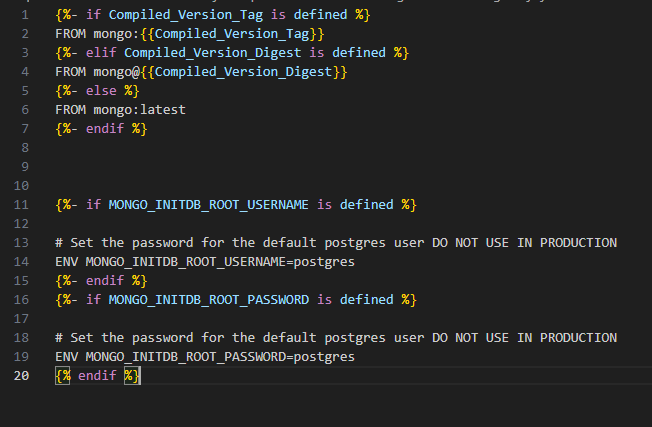
\includegraphics[width=0.75\textwidth]{jinja_template_database_mongodb.png}
	\caption{Ejemplo Plantilla para la configuración de un servicio de base de Datos para MongoDB.}
\end{figure}

Las plantillas tienen que tener la estructura necesaria de modo que, usando la Sintaxis de Jinja, el motor de plantillas sea capaz de crear un producto funcional para una configuración válida. La imagen de arriba puede ser parte de un solo componente de la plantilla.
Dividir las plantillas en componentes\footnote{Los componentes de una plantilla no son más que importar otros ficheros .jinja para dar estructura y evitar manejar un archivo gigante que recoja todas las opciones de configuración.} nos permite estructurar la plantilla; esto puede verse con un ejemplo en la Subsección \hyperref[sec:Plantilla Dockerfile]{Plantilla Dockerfile}.

\begin{figure}[h]
	\centering
		\includegraphics[width=0.75\textwidth]{Dockerfile.logica.plantillas.jinja.png}
	\caption{Ejemplo de división por componentes.}
\end{figure}


\newpage
\subsubsection{Mapping Model}
\label{sec:Mapping Model}
Es el único componente completamente opcional a la hora de resolver la variabilidad, tampoco es necesario crearlo para el desarrollo de las plantillas.

\begin{figure}[h]
	\centering
		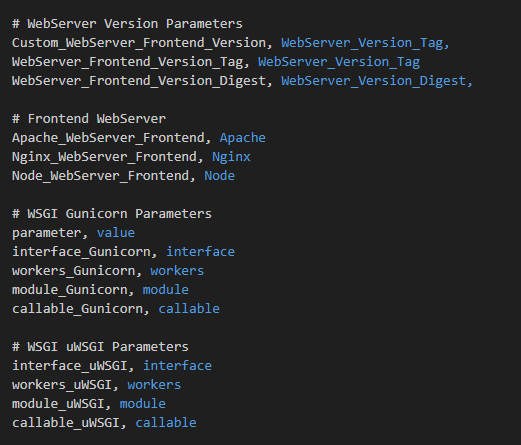
\includegraphics[width=0.75\textwidth]{mapping_model_screenshot.png}
	\caption{Ejemplo Mapping Model.}
\end{figure}

Contiene la estructura de un fichero csv de tres columnas. Las primeras columnas permiten mapear features sean estas booleanas o no, a otros features Booleanas que podrán ser empleadas en las plantillas Jinja, la tercera columna permite especificar una feature.
Este archivo permite renombrar features y hacerlas más comprensibles para las plantillas Jinja. También es el responsable de hacer funcionar configuraciones sobre otras plantillas.

\newpage
\subsection{Plantilla Dockerfile}
\label{sec:Plantilla Dockerfile}
Como hemos visto, un fichero Dockefile es un archivo de texto que contiene una serie de instrucciones que Docker \cite{docker} utilizará para construir una imagen de contenedor.
\subsubsection{Feature model}

La plantilla Dockerfile cuenta con el modelo más grande del proyecto. La idea para crear estos modelos de plantilla es subdividir el modelo en partes más pequeñas y manejables, de forma que se pueda trabajar con ellas de forma independiente.
El criterio a la hora de hacer subdivisiones es similar al criterio que usan repositorios como Docker Hub \cite{docker_hub} que divide sus imágenes por categorías dependiendo de su función.
En este contexto podemos construir una primera subdivisión que represente el resultado final esperado, es decir, la primera feature será decidir si nuestra imagen tiene el objetivo de desplegar un contenedor que albergue un servicio de Frontend, Backend, Base de datos, etc.

\begin{figure}[h]
	\centering
	  \includegraphics[width=0.5\textwidth]{Dockerfile.uvl.png}
	\caption{Captura de la primera subdivisión para Dockerfile.}
\end{figure}

Cada una de estas categorías contendrá a su vez una serie de subcategorías que representen las opciones de configuración que se pueden dar en cada una de ellas.
\\Centrémonos en el caso de uso de un Frontend. Comúnmente, al desplegar una imagen de Frontend, se sigue una estrategia de multietapa \cite{docker_multistage} donde en una primera etapa compilamos la aplicación 
y en una posterior etapa la alojamos en un servidor web, esto con el objetivo de crear una imagen lo más pequeña posible al no contener ninguno de los ficheros fuente.

\begin{figure}[h]
	\centering
	  \includegraphics[width=0.5\textwidth]{Dockerfile.frontend.png}
	\caption{Captura de las opciones de configuración para frontend.}
\end{figure}

En este caso las subcategorías podrían ser el lenguaje, el puerto en el que se desplegará la aplicación, el comando que se ejecutará al iniciar el contenedor, etc.
Estos son elementos ya mencionados en la sección de herramientas disponibles, como pueden ser las acciones del comando docker init en Docker Desktop \cite{docker_desktop}.  

Nuestro modelo permite recoger estas características además de otras,
como pueden ser el servidor web (Nginx, Apache, \ldots) que queremos junto con su versión, Podremos seleccionar el framework de desarrollo que se ha empleando, la versión en la que compilará la aplicación, etc.
Las posibilidades van mucho más allá de lo que se recoge en esta versión del fichero Dockerfile, pero estas opciones ya expanden enormemente la capacidad de configuración que tienen otras herramientas. 



\subsubsection{Plantillas Jinja2}
Una vez que contamos con el modelo de la plantilla, podemos proceder a la creación de las plantillas Jinja2 que son quienes realmente aportan el contenido al producto.

\begin{figure}[h]
	\centering
	  \includegraphics[width=0.5\textwidth]{Dockerfile.frontend.jinja.template.png}
	\caption{Captura Sección de la Plantilla Dockerfile. Podemos ver cómo la instrucción \texttt{EXPOSE} aparece en la plantilla Dockerfile a la hora de generar un producto con una configuración para exponer un servicio de frontend.}   
\end{figure}

La sintaxis de Jinja2 nos permite aplicar cierta lógica a la hora de generar los ficheros de configuración, por ejemplo, podemos emplear condicionales para que ciertas partes del fichero se generen o no en función de la configuración que se haya dado.
\begin{figure}[h]
	\centering
	  \includegraphics[width=0.5\textwidth]{Dockerfile.logica.plantillas.jinja.png}
	\caption{Captura de la primera subdivisión de la plantilla Dockerfile.}
\end{figure}

\newpage
Dividir las plantillas no solo es útil porque las hace más manejables y fáciles de mantener, sino que también permite la reutilización de las mismas. Por ejemplo, si tenemos una plantilla que se repite en varias plantillas, podemos extraerla a un fichero aparte y reutilizarla en todas las plantillas que lo necesiten.
Para este caso podemos generar una plantilla para los metadatos y labels\footnote{etiquetas} de la imagen. 

\begin{figure}[h]
	\centering
	  \includegraphics[width=0.5\textwidth]{Dockerfile.metadata.png}
	\caption{Captura de la primera subdivisión para Dockerfile.}
\end{figure}

\newpage

\subsubsection{Mapping Model}
El mapping model es un componente opcional que permite mapear features a otras features, esto es útil cuando queremos renombrar features o hacerlas más comprensibles para las plantillas Jinja.
En este caso, aplicamos dicha funcionalidad para paliar las restricciones actuales del parser existente del lenguaje UVL\footnote{En UVL no podemos emplear nombres de features que contengan espacios o caracteres especiales o bien tampoco podemos repetir nombres de features en varias partes del modelo}.
\begin{figure}[h]
	\centering
	  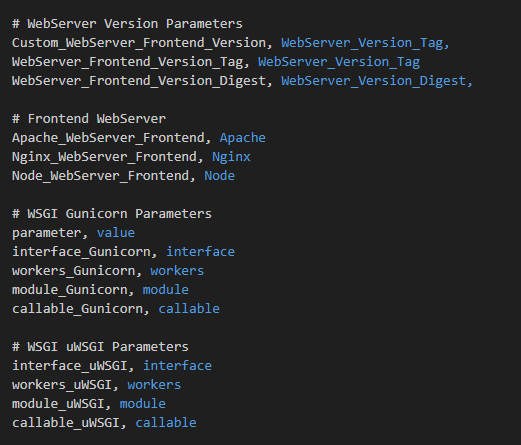
\includegraphics[width=0.5\textwidth]{mapping_model_screenshot.png}
	\caption{Captura de una sección del fichero Mapping Model plantilla Dockerfile.}
\end{figure}

\newpage

\subsubsection{Tests sobre la Plantilla Dockerfile}
El diseño y construcción de las plantillas es un proceso incremental, debe comprobarse con regularidad si la intención a la hora de seguir desarrollando una plantilla es mantener una coherencia con lo añadido hasta el momento. 

Con esta idea en mente, la solución propuesta consiste en la creación de pruebas que validen la correcta construcción de productos según la plantilla en la que estamos trabajando.

Estas pruebas deben ser capaces de comprobar que las plantillas generan un producto correcto. Para el caso del Dockerfile estas pruebas deben componerse de cada configuración y un producto esperado. Si nuestra plantilla es capaz de generar el mismo producto con la configuración dada de entrada, la prueba será considerada como exitosa. 

\begin{figure}[h]
	\centering
	  \includegraphics[width=0.75\textwidth]{Dockerfile.configuracion-backend.png}
	\caption{Configuración Ejemplo 1 Backend.}
\end{figure}

\newpage 

\begin{figure}[h]
	\centering
	  \includegraphics[width=1\textwidth]{Dockerfile.backend.producto.png}
	\caption{Producto Esperado para la configuración de la Figura 18.}
\end{figure}

Es evidente que ciertos cambios más radicales plantean refactorizar algunos test. 
Aun así, es aconsejable validar el diseño de los nuevos elementos de la plantilla solucionando estas incoherencias.
En el contexto de esta plantilla Dockerfile las pruebas se han realizado empleado las librerías de pytest \cite{pytest_docs} para la generación de los productos esperados. Estos test pueden encontrarse en el repositorio para el desarrollo de la plantilla dockerifle \cite{dockerfile_template_dev}.

\newpage
\subsubsection{Resto de Plantillas}
El proceso de creación de plantillas es similar para el resto de plantillas. La diferencia radica en la complejidad de las plantillas y en la cantidad de opciones de configuración que se pueden dar.
Estas plantillas pueden encontrarse en el repositorio \cite{m4rdom_templates}.














%% Arquitectura y Descripción del sistema Capitulo 6
\section{Arquitectura y Descripción del sistema }
\label{sec:Arquitectura y Descripción del sistema}
Esta sección describe la arquitectura y el modelado del sistema, incluyendo los componentes, la estructura y el diseño de la aplicación resultante en una imagen.
\subsection{Visión general de la arquitectura }
La arquitectura de la aplicación se divide en contenedores para manejar cada uno de los servicios de los que hace uso.
La aplicación se divide en 4 servicios principales: Repository-Manager, UVEngine-Resolver, Frontend y una instancia de nginx que hace de reverse proxy.
Podemos agrupar los contenedores de Repository-Manager y UVEngine-Resolver como el backend de nuestra aplicación.
Nuestro backend es responsable de la generación de los archivos de configuración a partir de las plantillas y de la comunicación con el repositorio de las plantillas.
Por otra parte, contamos con un servidor de nginx que ofrece nuestra aplicación Angular; a esta parte la llamaremos Frontend.
El frontend es responsable de la interacción con el usuario y la visualización de los archivos de configuración generados.
Como hemos mencionado anteriormente, también contamos con una instancia de Nginx que actúa como reverse proxy y que se encarga de enrutar las peticiones a los servicios de backend y frontend por comodidad en el desarrollo. 

\newpage 
\subsubsection{Diagrama de infraestructura}

\begin{figure}[h]
	\centering
	  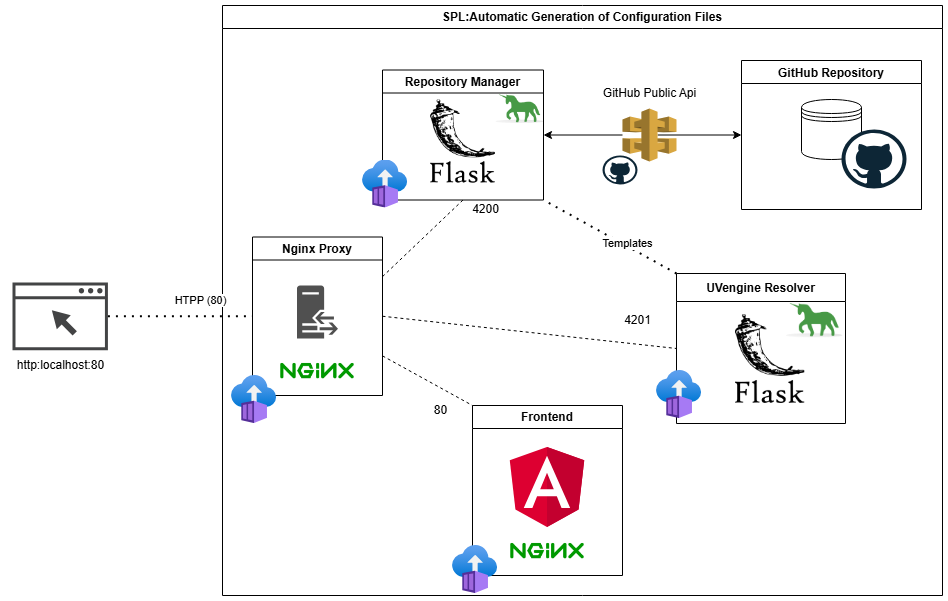
\includegraphics[width=1\textwidth]{Arquitectura Contenedores.png}
	\caption{Diagrama infraestructura de Contenedores.}
\end{figure}

\newpage
\subsection{Descripción de servicios de backend} 
El backend de nuestra aplicación se ha dividido en dos servicios independientes con el objetivo de simplificar el desarrollo de la aplicación.
Al contar con dos servicios independientes, podemos escalarlos de forma independiente y mantenerlos de forma independiente en un futuro si fuera necesario.


\subsubsection{Repository-Manager}
Este servicio se encarga de servir o traducir las peticiones que puede realizar el cliente o UVEngine-Resolver a la API de GitHub.
Estas peticiones son obtener el archivo .uvl de la plantilla seleccionada, obtener el listado de plantillas disponibles y obtener el listado de versiones disponibles para cada plantilla,
Esta aplicación está desarrollada en Python y emplea el framework Flask para la creación de la API, esta API se encarga de servir los archivos uvl de las plantillas y las versiones disponibles.
Para hacer funcionar esta API se emplea la API pública de GitHub que permite acceder al contenido de repositorios. 
En este caso el repositorio al que queremos acceder es el repositorio Templates \cite{m4rdom_templates} que contiene las plantillas disponibles.
También contamos con un Endpoint para descargar todo el contenido de las plantillas del repositorio. Este Endpoint es útil para mantener actualizadas las plantillas en el servidor UVengine Resolver.\footnote{En este momento es más eficiente descargar todo el repositorio de plantillas en una única petición para no abusar de la API pública de GitHub.}

\newpage
\subsubsection{UVEngine-Resolver}

El segundo servicio es UVEngine-Resolver, que se encarga de resolver la variabilidad a partir de recibir como parámetros un JSON que contiene el nombre de la plantilla, la versión a utilizar y la configuración. 
El resultado de la función será un JSON que contiene el producto generado a partir de la configuración dada. 
\begin{figure}[h]
	\centering
	  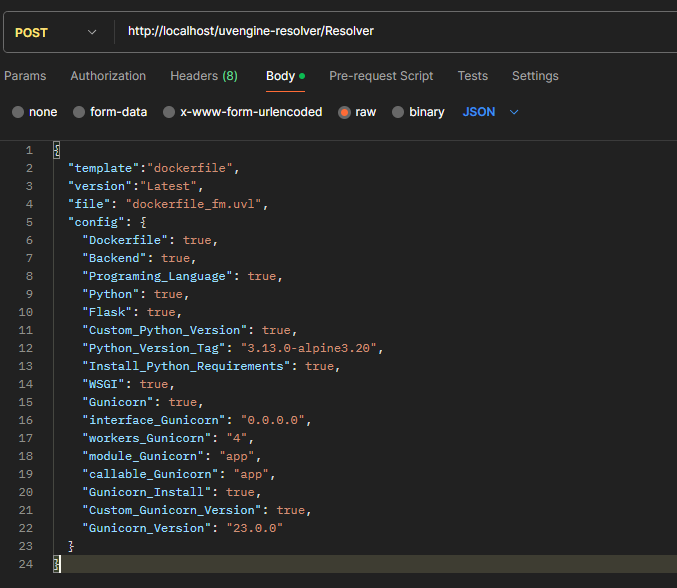
\includegraphics[width=1\textwidth]{Peticion POST uvengine-resolver.png}
	\caption{Ejemplo de una petición POST a UVEngine-Resolver.}
\end{figure}
\\
También contamos con algunos Endpoints que pueden recibirse tanto desde el cliente como del Servicio Repository-Manager para actualizar las plantillas.
\newpage
\subsection{Descripción de Frontend}
Como hemos comentado anteriormente, el Frontend es la parte de la aplicación que se encarga de la interacción con el usuario y la visualización de los archivos de configuración generados.
Se trata de una aplicación web desarrollada en Angular que permite al usuario seleccionar una plantilla y una versión y generar un producto a partir de una configuración válida.

La aplicación queda alojada en un contenedor de Docker que se encarga de servir la aplicación web en el puerto 80. Este contenedor se comunica con el servicio Repository-Manager para obtener las plantillas y versiones disponibles a través de peticiones del cliente.
Para servir la aplicación usamos el servidor web Nginx.













%% Extesivilidad de la aplicación
\section{Extensibilidad}
\label{sec:Extensibilidad}
En esta sección se pretende hacer hincapié en la extensibilidad de la aplicación.
Como se ha mencionado anteriormente, el proyecto tiene en mente que pueda adaptarse a las necesidades futuras.

Al almacenar las plantillas en un repositorio público de GitHub, permite a cualquier usuario modificar, añadir o eliminar plantillas de forma sencilla y ordenada.
Esto permite que el desarrollo de plantillas se maneje de forma independiente al resto de la aplicación y que se puedan añadir nuevas funcionalidades sin necesidad de modificar el código de la aplicación.
\subsection{Añadir Plantillas}
Existiendo varias formas en las que se pudiera haber diseñado la forma con la que añadir nuevas plantillas a la aplicación aprovechando características de GitHub, se ha optado por la solución más sencilla y directa.
Añadir una nueva plantilla es tan sencillo como añadir una nueva carpeta al repositorio de plantillas de GitHub,
Esta carpeta debe contener una estructura de directorios específica que contenga los archivos necesarios para la plantilla, como son el Feature Model en UVL, las plantillas Jinja2 y el archivo de Mapping Model; este último archivo es opcional.
Existen instrucciones detalladas de cómo añadir una plantilla al repositorio de plantillas.\footnote{Repositorio de plantillas: \url{https://github.com/M4rdom/Templates}.} o bien en el Apéndice \hyperref[sec:Manual de Desarrollo]{Manual de Desarrollo}.

\newpage

\subsubsection{Ampliar la Plantilla Dockerfile}
La plantilla Dockerfile recoge alguna de las características más interesantes que ya cubren otras herramientas, pero queda claro que todavía existe mucho margen de mejora en cuanto a la personalización de las opciones de configuración.
\\La plantilla no es a día de hoy capaz de cubrir todas las opciones de configuración que se pueden dar en un fichero Dockerfile, pero tiene el potencial de ser ampliada y mejorada en el futuro.
Ampliar esta plantilla es sencillo, se cuenta ya con un repositorio de desarrollo para la plantilla\footnote{Repositorio para el desarrollo de la Plantilla Dockerfile \url{https://github.com/M4rdom/Dockerfile-Template-Dev} \cite{dockerfile_template_dev}.} que contiene la plantilla y los test necesarios para validarla.
Una vez que se haya ampliado la plantilla, se puede añadir al repositorio de plantillas de GitHub y utilizarla para generar productos.
\\Al seleccionar una feature que no ha sido desarrollada, el producto resultante (en este caso el fichero Dockerfile) contendrá el siguiente mensaje de error:

\begin{figure}[h]
	\centering
	  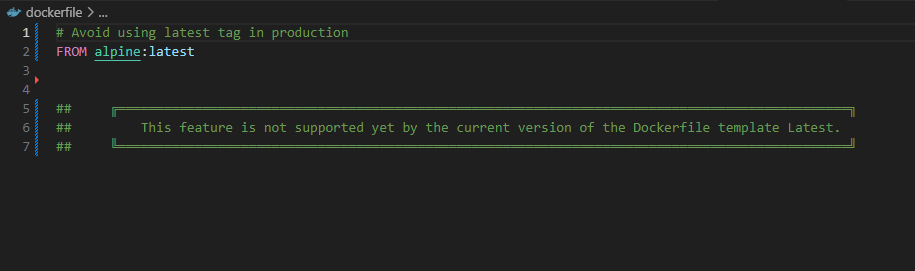
\includegraphics[width=1\textwidth]{unupportedfeature.png}
	\caption{Mensaje de Error en el Producto Final.}
\end{figure}








%% Despliegue de la aplicación
\section{Despliegue de la aplicación }
\label{sec:Despliegue de la aplicación}
\subsection{Despliegue local}
Para desplegar el proyecto y todas sus capas se hace uso de la herramienta Docker, que permite la creación de contenedores ligeros y portables que pueden ejecutarse en cualquier entorno.
Para el despliegue local se hace uso de Docker Compose \cite{docker_desktop}, que permite definir y ejecutar aplicaciones Docker multicontenedor generando todos los servicios necesarios para el despliegue de la aplicación.
Esto supone una abstracción de la infraestructura necesaria para el despliegue de la aplicación, permitiendo la creación de un entorno de desarrollo y pruebas aislado y reproducible.
En el proyecto se encuentra el fichero docker-compose.yml que contiene la configuración necesaria para el despliegue de la aplicación en un entorno local.
\begin{verbatim}
	version: '3.8'

	services:
	  fronted:
		build:
		  context: ./Frontend
		  Dockerfile: Dockerfile
		container_name: frontend
		ports:
		  - "4200:80"
	  
	  repository-manager:
		build:
		  context: ./Repository-Manager
		  Dockerfile: Dockerfile
		container_name: repository-manager
		ports:
		  - "5000:5000"
	
	  uvengine-resolver:
		build:
		  context: ./UVEngine-Resolver
		  Dockerfile: Dockerfile
		container_name: uvengine-resolver
		ports:
		  - "5001:5001"
		depends_on:
		  - repository-manager
	  
	  nginx-reverse-proxy:
		build:
		  context: ./Nginx-Reverse-Proxy
		  Dockerfile: Dockerfile
		container_name: nginx-reverse-proxy
		ports:
		  - "80:80"
	\end{verbatim}

Como se observa, el código se compone de 4 servicios:
\begin{itemize}
	\item Frontend: Servicio que se encarga de servir la aplicación web.
	\item Repository Manager: Servicio que se encarga de servir los archivos UVL de las plantillas y las versiones disponibles.
	\item UVEngine Resolver: Servicio que se encarga de resolver la variabilidad a partir de recibir como parámetros un fichero JSON que contiene el nombre de la plantilla, la versión a utilizar y la configuración.
	\item Nginx Reverse Proxy: Servicio que se encarga de redirigir las peticiones de la aplicación web al servidor de backend y frontend.	
\end{itemize}

La instrucción dockercompse up creará los contenedores en la configuración ya escrita. La web será accesible en la dirección localhost en el puerto 80.





%% Resultados
\section{Resultados}
\label{sec:Resultados}
Esta parte del documento se centra en los resultados obtenidos durante el desarrollo del proyecto, incluyendo los resultados de las pruebas, la viabilidad del proyecto y la escalabilidad.
\subsection{Resultados Obtenidos}
Cumpliendo los objetivos propuestos al inicio del proyecto, se ha desarrollado una aplicación que permite la generación automática de archivos de configuración a partir de plantillas.

Un resumen de los resultados del proyecto es el siguiente:

\begin{itemize}
\item La plataforma web de la aplicación aporta una forma ágil de crear productos software a partir de ellas.

\item Las plantillas para generar ficheros como Dockerfiles recogen un interesante número de posibilidades, entre las que se encuentran las opciones más usadas. Una vez generamos una configuración, podemos simplemente descargar el fichero generado o copiarlo al portapapeles y quedaría listo para su uso.

\item El empleo de la extensión UVLS para generar una configuración puede ser muy eficiente a la hora de generar productos con opciones de configuración relacionadas entre sí.
Además, tenemos la posibilidad de editar el producto final antes de utilizarlo.

\item Las plantillas existentes aportan unas funcionalidades interesantes que pueden explotarse a la hora de generar productos como ficheros de configuración.

\item El repositorio es fácilmente ampliable para abarcar nuevas plantillas y desarrollar nuevas funcionalidades.
\end{itemize}

\newpage 

Resumen de los desarrollos resultantes del proyecto:
\begin{itemize}
	\item Se ha desarrollado una aplicación web que permite la interacción con el usuario y la visualización de los archivos de configuración generados.
	\item Se adaptado el uso del proyecto UVEngine que permite la generación automática de archivos de configuración a partir de plantillas, adaptándola a las necesidades del proyecto.
	\item Se ha desarrollado una aplicación de Repository-Manager que permite la comunicación con el repositorio de plantillas de GitHub. \cite{m4rdom_templates} .
	\item Se ha desarrollado una aplicación de UVEngine-Resolver que permite la resolución de la variabilidad a partir de una configuración.
	\item Se ha creado la plantilla para la generación de ficheros Dockerfile a partir de una configuración, además de un entorno de desarrollo para la misma.
	\item Se ha desarrollado plantillas auxiliares para ficheros de configuración Nginx, dockerignore, etc.
	\item Se han desarrollado pruebas para validar la correcta construcción de los productos a partir de las plantillas Dockerfile.
	\item Se ha aportado todo el código fuente y la documentación necesaria para la replicación del proyecto.
	\item Se ha generado una Memoria que documenta todo el proceso de desarrollo.
	\item Se han aportado apéndices para el uso más fundamental de la aplicación.
\end{itemize}

\subsection{Viabilidad del proyecto}
Como hemos recogido arriba, el proyecto es potencialmente viable, pero presenta algunas carencias que pueden ser corregidas.
Es posible que el uso obligatorio de la extensión UVLS para generar los ficheros de configuración sea un punto en contra para la viabilidad del proyecto, 
El uso de la herramienta de configuración puede no estar a la altura en cuanto a comodidad de uso de otras herramientas de generación automática de archivos.
Las soluciones actualmente disponibles son más cómodas al detectar las features del proyecto de forma autónoma, sin necesidad de intervención del usuario. Esto supone que esta solución quede atrás en cuanto a comodidad. 
Es conveniente adaptar este sistema para que sea capaz de detectar algunas de las features de forma autónoma y dejar otras para la personalización del usuario, al menos en cuanto nos referimos a la generación del fichero Dockerfile.

\subsection{Escalabilidad}
Teniendo en cuenta que la escalabilidad de cualquier aplicación depende de la capacidad de sus servicios de generar nuevas instancias, es en un principio viable,
escalar horizontalmente cada uno de los servicios. Sin embargo, la escalabilidad de la aplicación se ve limitada actualmente por el uso de API pública de GitHub \cite{github_rest_api} para el servicio de Repository-manager visto en el \hyperref[sec:Desarrollo de los servicios de backend]{Capítulo 6} que limita el número de peticiones que se pueden hacer en un periodo de tiempo.\footnote{Actualmente el número de peticiones que puede realizarse a la API son 80 peticiones por minuto; esto es propenso a que cambien en un futuro.}
En el escenario en el que se quiera llevar la aplicación a un entorno de producción, debe sortearse este problema bien por medio del uso de tokens de autenticación.
Existe la posibilidad de que el usuario aporte un token personal de una cuenta de GitHub a la hora de desplegar el servicio o bien emplear un token propio desde GitHub.

En el escenario de superar dicho límite, desde la aplicación no se podrá descargar modelos UVL ni se podrá recargar el listado de plantillas ni versiones de las mismas.
No obstante, se podrá resolver la variabilidad de las plantillas que ya se han descargado y se podrá generar productos a partir de ellas si se encuentran disponibles en el servidor de backend, gracias al UVEngine-Resolver. 










%% Conclusiones
\section{Conclusiones y líneas futuras}
\label{sec:Conclusiones}


\subsection{Conclusiones del Desarrollo del proyecto}
El desarrollo del proyecto ha permitido alcanzar los objetivos planteados inicialmente. Se ha logrado implementar una solución eficiente y potencialmente escalable que cumple con los requisitos funcionales y no funcionales establecidos. Además, se ha adquirido un conocimiento profundo sobre las tecnologías utilizadas y se han identificado áreas de mejora para futuros desarrollos.
El desarrollo de las plantillas ha sido conservador y no se ha considerado explorar más que casos básicos de uso. Esto era algo esperado si asumimos la gran casuística que tenemos. Sin embargo, se ha demostrado que la aplicación es capaz de generar productos válidos a partir de configuraciones válidas. Dado el nivel de desarrollo de las herramientas (UVLS) y tecnologías de las que hace uso este trabajo se ha demostrado que es posible llevar a cabo un proyecto de estas características.
\subsection{Conclusión Personal}
A nivel personal, el desarrollo de este trabajo me ha servido para introducirme de lleno en la tecnología de contenedores, cómo esta tecnología se aplica en servicios y qué implicaciones existen a nivel de rendimiento y seguridad. Considero que el proyecto tiene de base una serie de fortalezas que otra serie de herramientas no consigue ofrecer actualmente. Es posible que un proyecto más ambicioso y con más recursos pueda explotar estas fortalezas y llevar el diseño de productos por este camino.
Sin duda, el proyecto queda lejos de tener aplicaciones funcionales reales, pero muestra un camino que puede ser explotado si se considera. 
\subsection{Aplicaciones Prácticas}
Además de contar con una forma interesante de generar Dockerfiles, pueden existir dinámicas para aprovechar configuraciones válidas para generar otros ficheros necesarios, como, por ejemplo, podemos generar ficheros de configuración para el servidor de Nginx \cite{nginx} directamente a partir de la configuración para generar un Dockerfile. 
Esto es gracias a los ficheros Mapping Models y a un diseño inteligente de las plantillas.
\subsection{Desarrollo de nuevas plantillas}
El proyecto está preparado para recibir nuevas plantillas manteniendo las existentes, por ejemplo, pueden agregarse todo tipo de plantillas que requieran de la salida de un fichero de configuración, como pueden ser en el caso de herramientas como Ansible \cite{ansible}.	 
Una vez añadidas plantillas al repositorio, éstas estarán disponibles de la misma forma en la que están disponibles las plantillas existentes y solo será necesario recargar el listado de plantillas que se encuentra en la barra de navegación de la aplicación web.	
\subsection{Continuación en el desarrollo de plantillas ya existentes}
Las plantillas existentes tienen un gran margen de mejora. En la situación actual no soportan la gran mayoría de las opciones de configuración que se pueden dar en un fichero Dockerfile. Además, las opciones que se manejan son propensas a quedar obsoletas y se necesita de una continua revisión de las plantillas en busca de problemas de diseño o seguridad.
Estos son problemas que padecen otras herramientas que nos permiten generar el ficheros Dockerfile de forma automática.

\subsection{Mejorar la experiencia del usuario }
La generación de la configuraciones está ligada al desarrollo de la extensión UVLS. Dicha extensión permite al usuario generar una configuración válida desplegando el árbol de características, pero para ello el usuario
necesita contar con VS Code y la extensión instalada para ser capaz de generar configuraciones válidas. La propuesta para este escenario sería la integración de dicha funcionalidad dentro de la plataforma web,
La extensión UVLS es un proyecto de código abierto y su integración en la aplicación web podría ser un proyecto en sí mismo. 

En el desarrollo del trabajo se ha explorado esta posibilidad ejecutando dicha extensión en la versión web del editor VS Code, pero el resultado en cuanto a rendimiento hace que esta opción no sea viable.

La propia aplicación web puede ser mejorada en cuanto a la experiencia del usuario, añadiendo más información al usuario para colocar más contexto a la hora de seleccionar una plantilla y las posibilidades de combinar configuraciones. 
Otras opciones que pueden explorarse serían llevar la aplicación a un entorno de escritorio empleando Electron \cite{electron}.

Otras mejoras que supondrían una gran aportación serían desarrollar herramientas que permitan la generación de configuraciones de forma automática reconociendo las necesidades del proyecto, como hacen otras aplicaciones como Starter \cite{starter}.

\subsection{Mejorar la escalabilidad de la aplicación}
La escalabilidad de la aplicación se ve limitada por el uso de la API pública de GitHub para el servicio de Repository-manager.
Por tanto, adaptar la aplicación a peticiones autorizadas a la API de GitHub es una mejora necesaria para llevar la aplicación a un entorno de producción.






%%%% Sections
%%\section{One \\}
%%
%%\subsection{Motivation}
%%    \blindtext[2]
%%    
%%    \begin{figure}[ht]
%%      \centering
%%        
\includegraphics[width=0.5\textwidth]{xp}
%%      \caption{A diagram showing the iterations of extreme programming.}
%%    \end{figure}
%%    
%%    \blindtext[4]
%%
%%\section{Two \\}
%%    \blindmathpaper






% Imprimir la bibliografía
\printbibliography




%% Bibliografia
%%\begin{thebibliography}{9}
%%    \bibitem{latexcompanion} 
%%    Michel Goossens, Frank Mittelbach, and Alexander Samarin. 
%%    \textit{The \LaTeX\ Companion}. 
%%    Addison-Wesley, Reading, Massachusetts, 1993.
%%    
%%    \bibitem{einstein} 
%%    Albert Einstein. 
%%    \textit{Zur Elektrodynamik bewegter K{\"o}rper}. (German) 
%%    [\textit{On the electrodynamics of moving bodies}]. 
%%    Annalen der Physik, 322(10):891–921, 1905.
%%\end{thebibliography}




%%\end{document}















%% Apendices

\begin{umaappendices}
    \section{Manual de \\ Instalación}
	\label{sec:Manual de Instalación}
	\subsection{Requisitos Previos}
	Para lanzar la aplicación en un entorno local, debemos contar con los siguientes requisitos previos:
	\begin{itemize}
		\item Navegador Web
		\item Docker
		\item Visual Studio Code con la extensión UVLS \cite{uvls_code} instalada.
		\item Git
	\end{itemize}

	\subsection{Descargar el código fuente}
	Para descargar el código fuente de la aplicación, debemos clonar el repositorio de GitHub \cite{m4rdom_project_repository}\footnote{https://github.com/M4rdom/Automatic-generation-of-configuration-files-for-deploying-services-in-Docker} en un directorio local.
	usando la instrucción \texttt{git clone} o bien descargar el repositorio en formato zip.
	\subsection{Despliegue del Servicio}
	Para desplegar el servicio debemos situarnos en la raíz del proyecto y ejecutar el siguiente comando:
	\begin{verbatim}
		docker-compose up
	\end{verbatim}
	\subsection{Acceso a la aplicación}
	Una vez que los servicios se hayan desplegado correctamente, podremos acceder a la aplicación web en la dirección localhost en el puerto 80.
	\begin{figure}[ht]
		\centering
			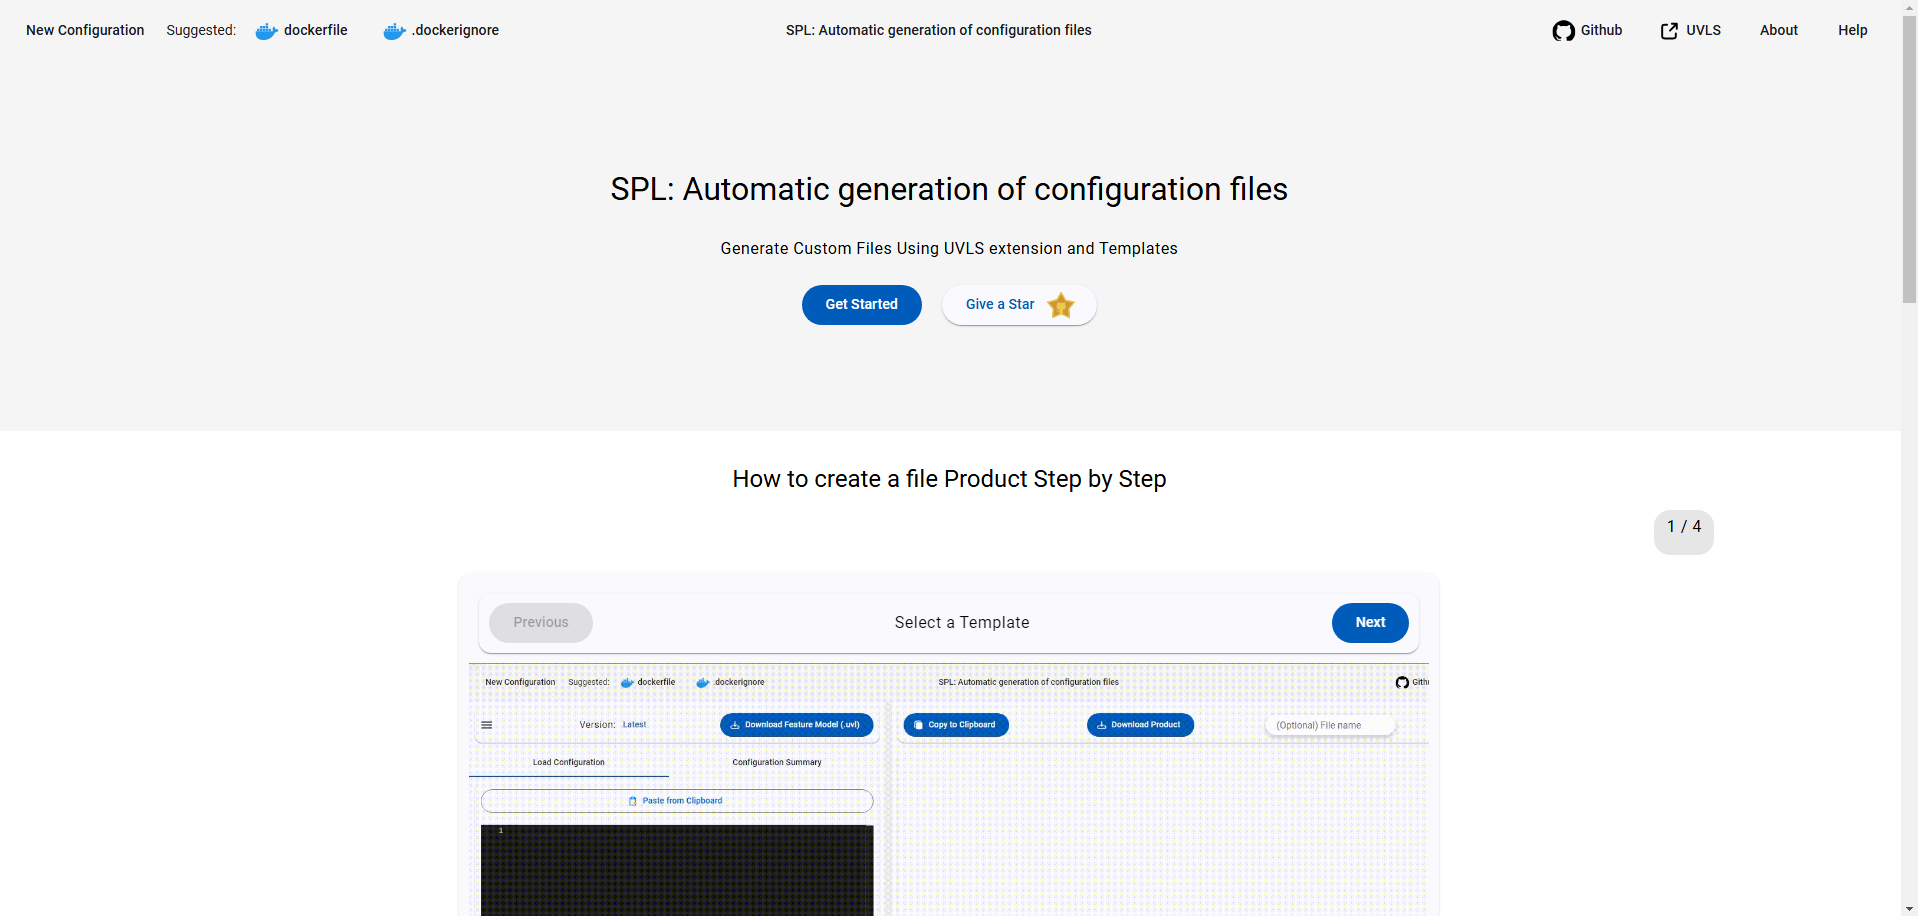
\includegraphics[width=0.5\textwidth]{frontpage.png}
		\caption{Página Principal}
	\end{figure}
	\subsubsection{GitHub API}
	Debemos recordar que la aplicación hace uso de la API pública de GitHub \cite{github_rest_api} para el servicio de Repository-manager, por lo que es posible que se alcance el límite de peticiones permitidas por la API.
	Para superar este límite se puede emplear un token de autenticación de GitHub \cite{github_tokens} para aumentar el número de peticiones permitidas.
	Para un uso estándar no es necesario emplear un token de autenticación.
	\subsection{Terminar el servicio}
	Para terminar el servicio debemos ejecutar el siguiente comando en la raíz del proyecto:
	\begin{verbatim}
		docker-compose down
	\end{verbatim}



    \section{Manual de Uso}
	\label{sec:Manual de Uso}
	\subsection{Inicio de la aplicación}
	Para iniciar la aplicación debemos acceder a la dirección localhost en el puerto 80.
	\begin{figure}[ht]
		\centering
			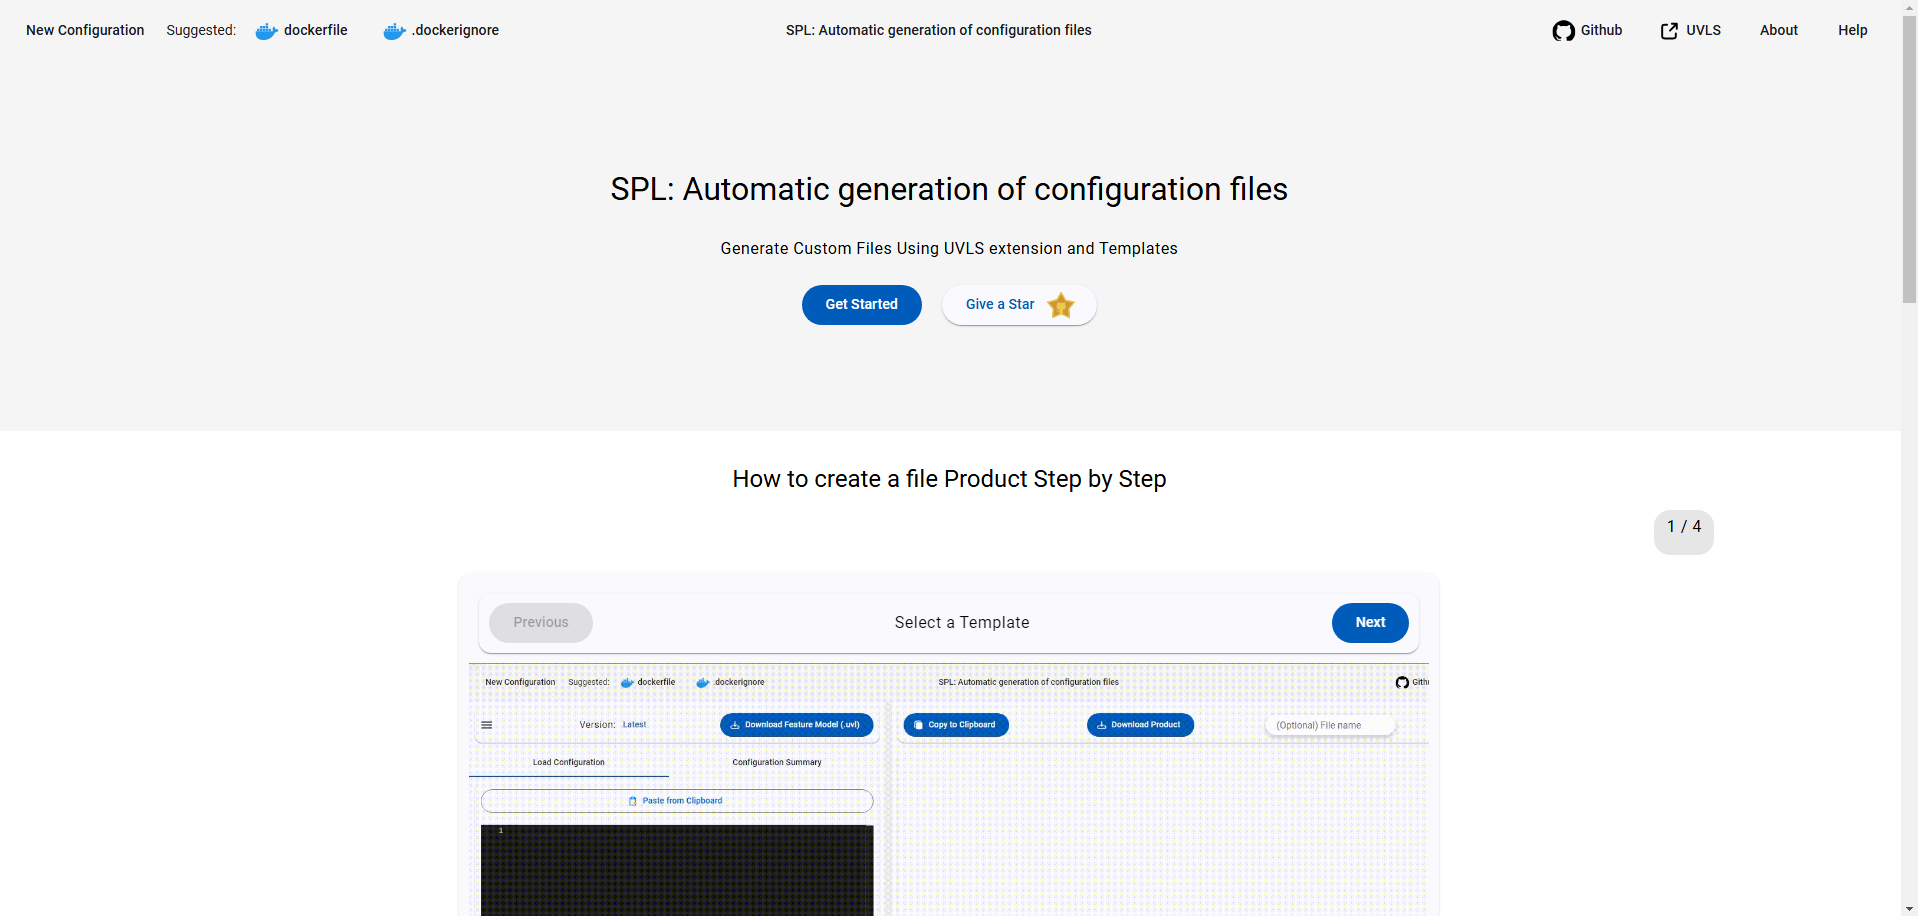
\includegraphics[width=1\textwidth]{frontpage.png}
		\caption{Página Principal.}
	\end{figure}
	\subsection{Barra de Navegación}
	La barra de navegación de la aplicación web contiene las siguientes opciones:
	\begin{figure}[ht]
		\centering
			
\includegraphics[width=1\textwidth]{navpage.png}
		\caption{Página Principal.}
	\end{figure}
	\begin{itemize}
		\item 	New Configuration: Permite al usuario seleccionar una plantilla y una versión y generar un producto a partir de una configuración válida.
		\item 	Dockerfile: Permite al usuario crear un Dockerfile a partir de una configuración válida.
		\item 	.dockerignore: Permite al usuario crear un fichero .dockerignore a partir de una configuración válida.
		\item 	SPL: Automatic Generation of Configuration Files for Deploying Services in Docker: Permite al usuario acceder a la página principal.
		\item 	GitHub: Link a la página de GitHub del proyecto.
		\item 	UVLS: Link a la extensión UVLS en el Visual Studio Code Marketplace.
		\item 	About: Página con información sobre el proyecto.
		\item 	Help: Página con información sobre cómo usar la aplicación.
	
	\end{itemize}

	

	\subsection{Seleccionar plantilla}
	Para seleccionar una plantilla debemos acceder a la página New Configuration y seleccionar una plantilla de la lista desplegable.

	\begin{figure}[h]
		\centering
			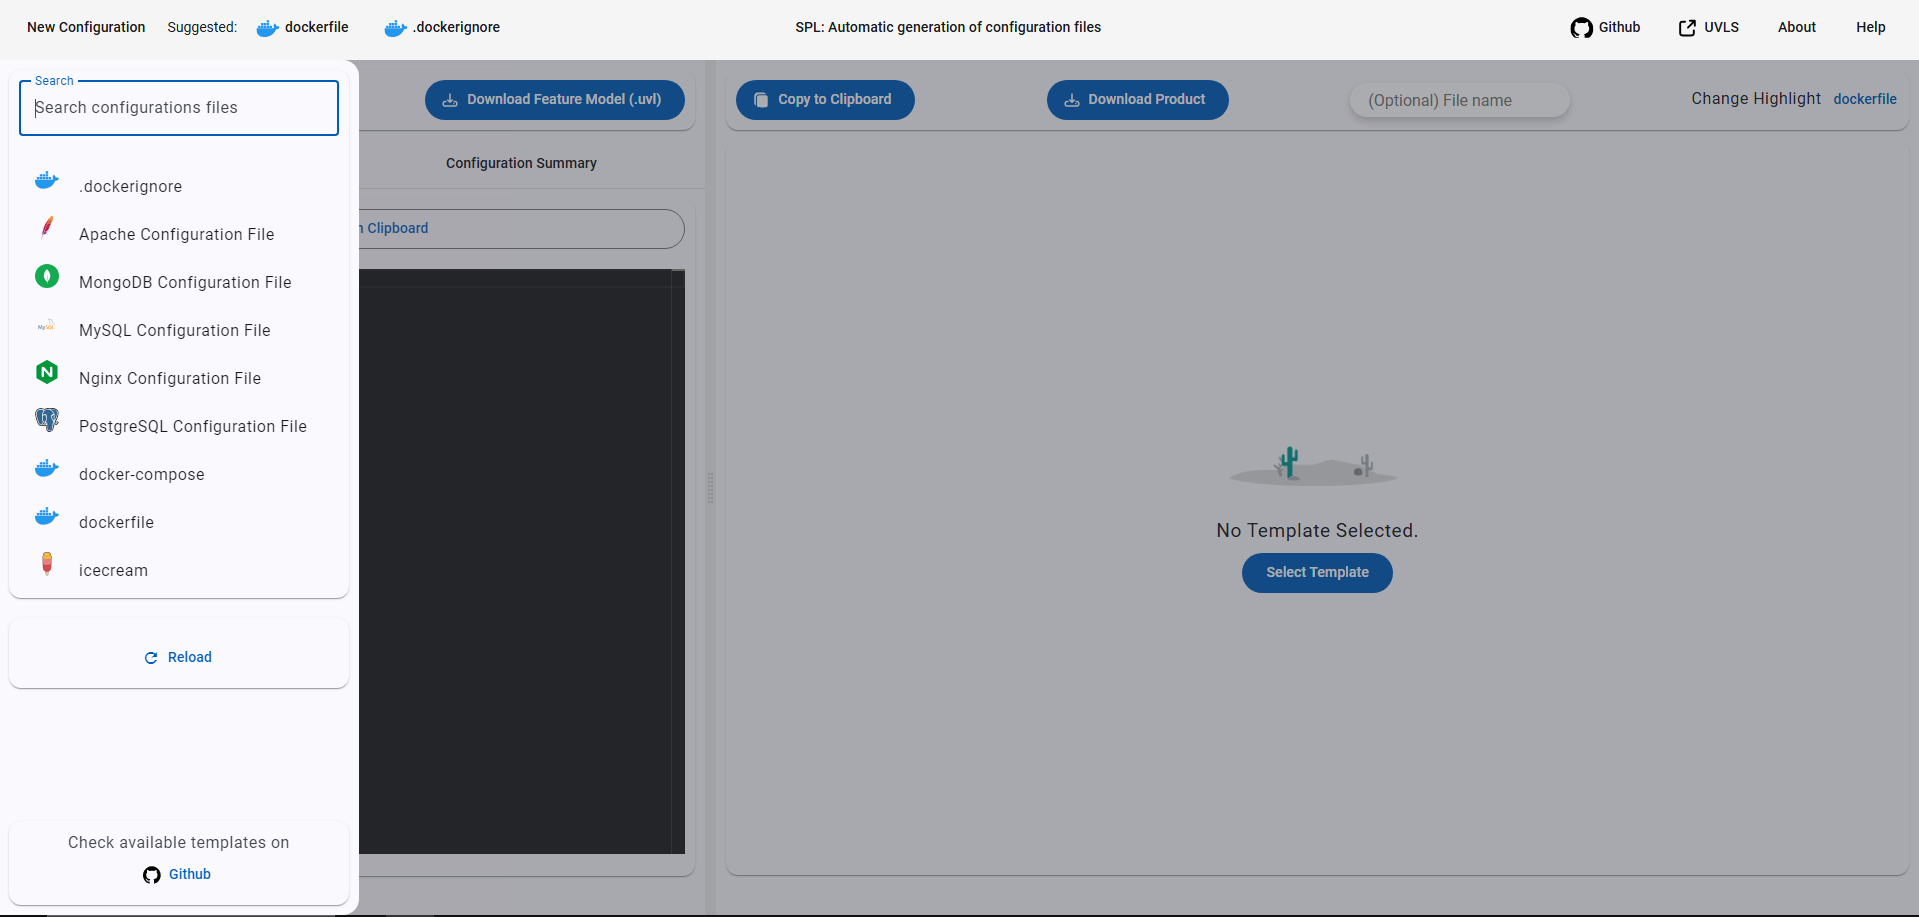
\includegraphics[width=1\textwidth]{selectTemplatePage.png}
		\caption{Barra Desplegable Selector de Plantillas.}
	\end{figure}
	\newpage
	\subsubsection{Seleccionar versión de la plantilla}
	Para seleccionar la versión de la plantilla, abrimos el desplegable Version; por defecto tiene el valor de Latest.
	\begin{figure}[h]
		\centering
			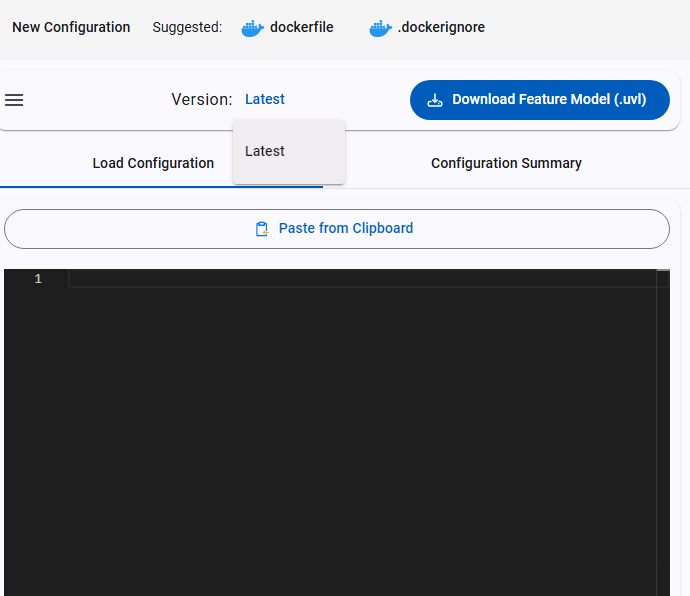
\includegraphics[width=0.75\textwidth]{selectionVersion.png}
		\caption{Captura Versiones Disponibles.}\footnote{En la imagen se muestra únicamente la versión Latest. Otras plantillas pueden contener más versiones que esta.}
	\end{figure}

	\newpage

	\subsubsection{Refrescar Plantillas}
	\label{sec:Actualizar Plantillas}
	En la página de arriba tendremos la opción de actualizar la lista de plantillas disponibles haciendo clic en el botón Reload.

	\begin{figure}[h]
		\centering
			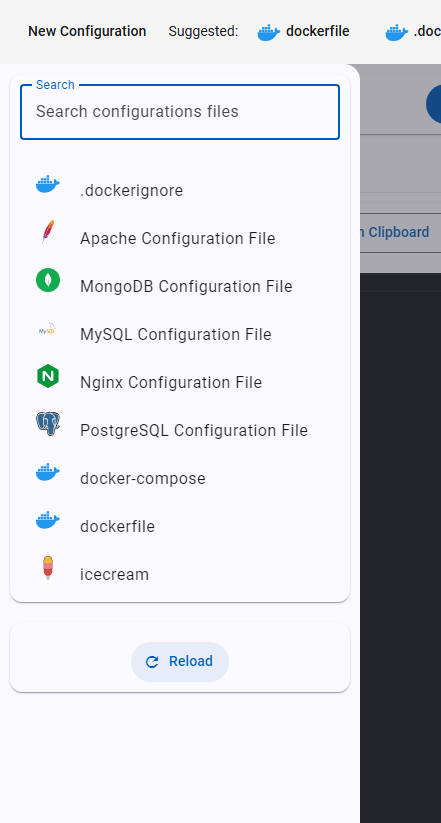
\includegraphics[width=0.4\textwidth]{RefreshTemplates.png}
		\caption{Captura Versiones Disponibles.}
	\end{figure}

	\subsubsection{Cargar configuración}
	Para cargar una configuración debemos hacer clic en el botón Load Configuration y copiar en el editor un fichero de configuración valido,
	opcionalmente, podemos pegar la configuración desde el portapapeles.
	\begin{figure}[h]
		\centering
			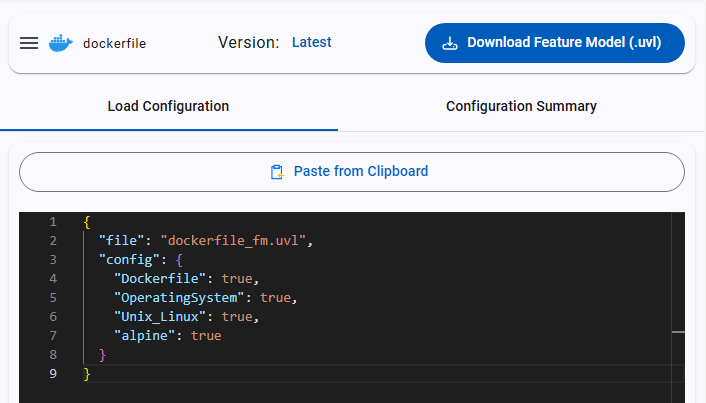
\includegraphics[width=0.75\textwidth]{loadconfiguration.png}
		\caption{Editor para cargar configuración,}
	\end{figure}
	\newpage

	\subsubsection{Descargar Fichero Generado}
	Una vez que hemos cargado la configuración y seleccionado una plantilla y una versión, podemos descargar el fichero generado haciendo clic en el botón Download File y opcionalmente añadiendo un nombre al fichero de salida. O bien simplemente copiamos al portapapeles.
	\begin{figure}[h]
		\centering
			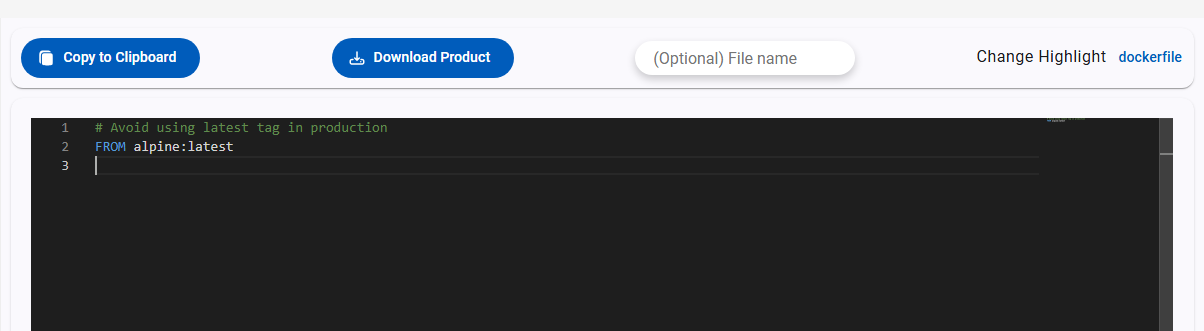
\includegraphics[width=1\textwidth]{donwloadToolbar.png}
		\caption{Editor para guardar Configuración.}
	\end{figure}


	\newpage
	\subsubsection{About Page}
	About Page contiene información sobre el proyecto, el motivo de su existencia, los objetivos que pretende alcanzar y su desarrollador.
	\begin{figure}[h]
		\centering
			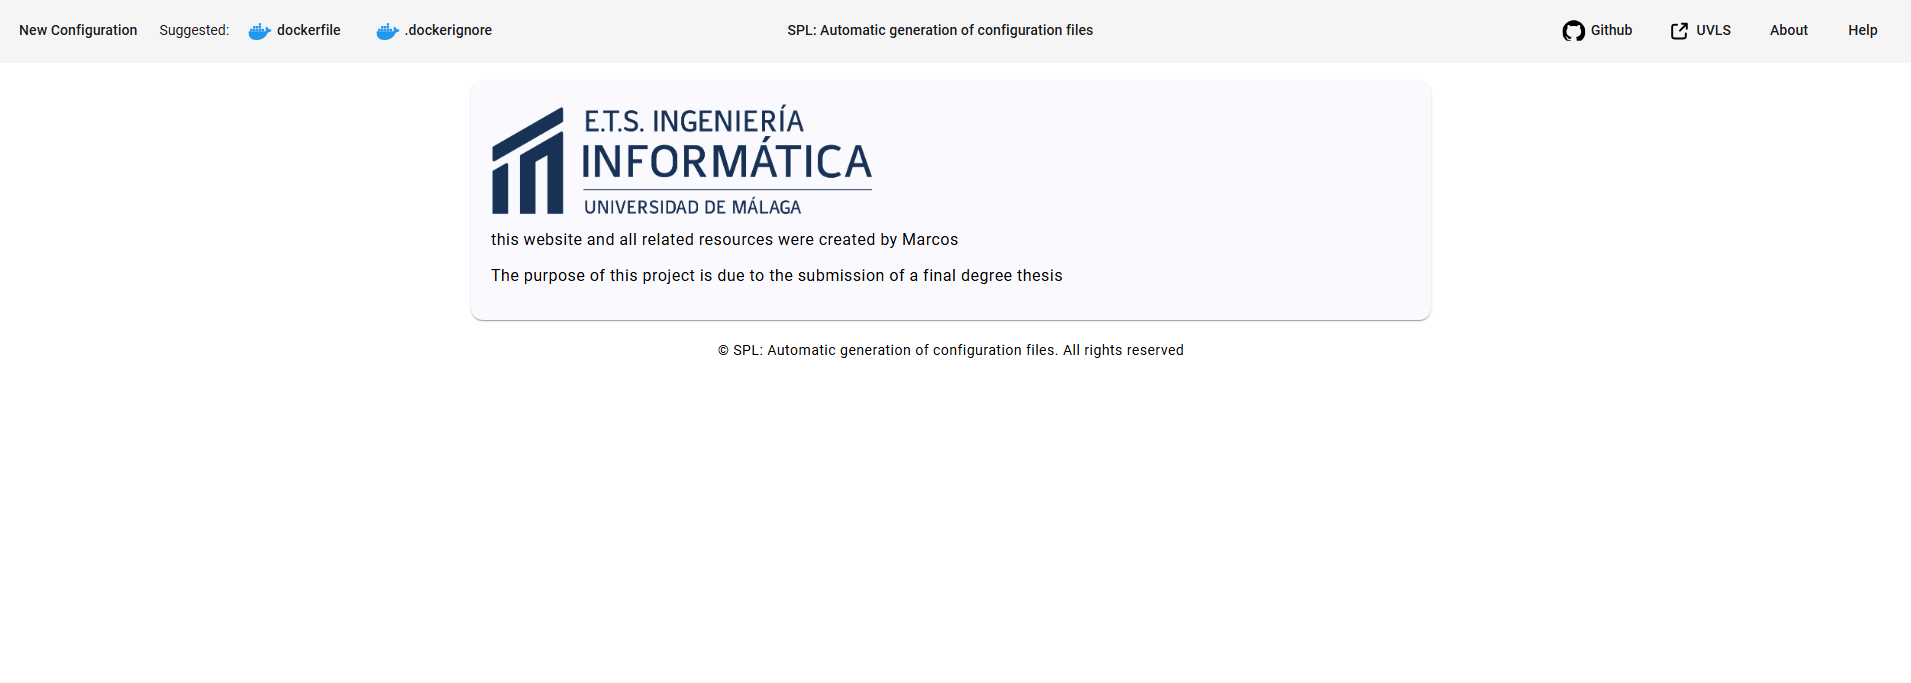
\includegraphics[width=1\textwidth]{Aboutpage.png}
		\caption{Página Principal.}
	\end{figure}

	\subsubsection{Help Page}
	Help Page contiene información sobre la terminología del proyecto. 
	\begin{figure}[h]
		\centering
			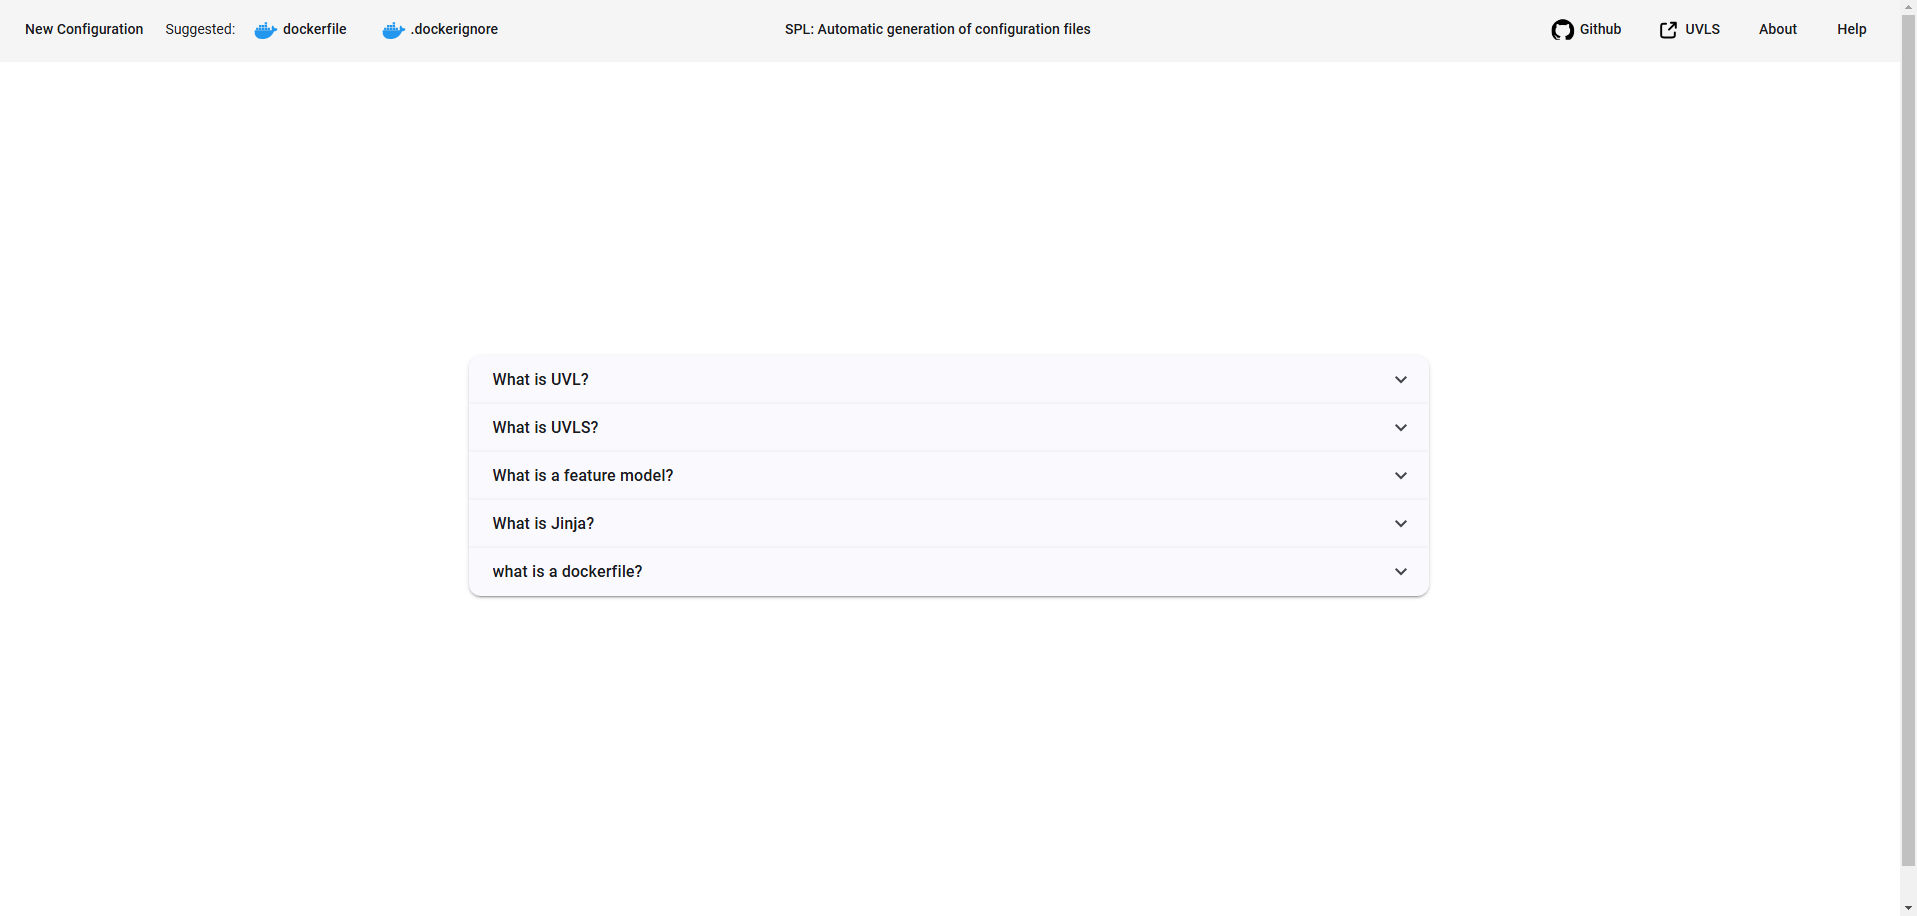
\includegraphics[width=1\textwidth]{HelpPage.png}
		\caption{Captura Página de ayuda.}
	\end{figure}




	\section{Manual desarrollo de plantillas}
	\label{sec:Manual de Desarrollo}
	\subsection{Introducción}
	Este manual describe los pasos necesarios tanto para añadir nuevas plantillas al repositorio de plantillas \cite{m4rdom_templates} como para modificar las plantillas existentes.
	una vez añadidas las plantillas al repositorio, será necesario actualizar la lista de plantillas dentro de la aplicación; véase el \hyperref[sec:Actualizar Plantillas]{Manual de Uso}.
	\subsubsection{Como añadir nuevas plantillas al repositorio}
	Para añadir una nueva plantilla al repositorio de plantillas debemos seguir los siguientes pasos:
	\begin{itemize}
		\item Generar la Estructura de directorios apropiada para la plantilla:
		\begin{itemize}
			\item Crear una carpeta con el nombre de la plantilla.
			\item Dentro de la Carpeta, Crear una carpeta con el nombre de la versión.
			\item Dentro del nuevo Directorio, Crear las Carpetas Feature Model, Jinja Templates y opcionalmente Mapping Model.
		\end{itemize}
		\item Añadir el archivo con nombre \"<Nombre de la Plantilla>\_fm.uvl" dentro del directorio Feauture Model.
		\item Añadir las plantillas Jinja a la carpeta Jinja Templates, la plantilla principal debe estar bajo el nombre \"<Nombre de la Plantilla>.jinja".
		\item (Opcional) Añadir el archivo de Mapping Model  a la carpeta Mapping Model bajo el nombre \"<Nombre de la Plantilla>\_mapping\_model.csv".
		\item Subir la plantilla al repositorio de plantillas haciendo push al repositorio.
		\item Actualizar la lista de plantillas en la aplicación web.
	\end{itemize}
	\subsubsection{Estructura de directorios}
	 A modo de resumen, la estructura de directorios de una plantilla debe ser la siguiente:

	\dirtree{%
	.1 /Template\_Name.
	.2 /Version\_Name.
	.3 /Feature Model.
	.4 Template\_Name\_fm.uvl.
	.3 Jinja Templates.
	.4 /More Jinja Templates (Optinal).
	.4 Template\_Name.jinja.
	.3 /Mapping Model (Optinal).
	.4 Template\_Name\_mapping\_model.csv.
}


	\subsubsection{Modificar las plantillas del repositorio}
	En el caso de que queramos modificar una plantilla ya existente en el repositorio de plantillas, debemos seguir los siguientes pasos:
	\begin{itemize}
		\item Modificar los archivos de la plantilla que queremos modificar respetando la estructura y nombres de la plantilla.
		\item Solicitar Pull Request al repositorio de plantillas
		\item Actualizar la lista de plantillas en la aplicación web.
	\end{itemize}

	Es recomendable generar estas plantillas a partir de un repositorio de desarrollo \cite{dockerfile_template_dev} para asegurar que las plantillas generan productos válidos realizando pruebas.
	Una vez que tengamos una plantilla lista, es solo cuestión de subirla al repositorio respetando la estructura original modificando únicamente la única plantilla que se desea modificar.
	Estas Instrucciones pueden verse con más detalle en el repositorio de plantillas \cite{m4rdom_templates}.




\end{umaappendices}

%% Back Cover

\includepdf[noautoscale=true, width=\paperwidth]{Portada-Titulo-Contraportada/backcover.pdf}
\end{document}



\end{document}